% !TeX spellcheck = en_US
\documentclass[12pt, fleqn, titlepage]{article}
%\usepackage{siunitx}
\usepackage{SpeedyGonzales}
\usepackage{MediocreMike}
\newcommand{\so}[2]{{#1}\mathrm{e}{#2}}
% \geometry{top=1cm}
%\usepackage{cleveref}
\usepackage{hyperref}
\usepackage{array}
\usepackage{amsmath}
\usepackage{ragged2e}
\usepackage{booktabs}
\usepackage{lipsum}
\usepackage{csquotes}
\usepackage{longtable}
\usepackage{arydshln}
\usepackage{subcaption}
\usepackage{listings}
\usepackage{pxfonts}
\usepackage{array}
\usepackage{multirow}
\usepackage{enumitem}
\usepackage{color}
\usepackage{booktabs}
\usepackage{makecell}
\usepackage{multicol}
\usepackage{nccmath}
\usepackage{graphicx}

\hypersetup{
	colorlinks=true,
	linkcolor=blue,
	filecolor=magenta,      
	urlcolor=cyan,
}

% Variables for result plots
\newcommand\skipper{1.4pt}
\newcommand\ripper{2.5pt}

\title{CycleGAN for Removing Field Strength Bias in Alzheimer's Disease Classification Model}
\author{Oskar Eiler Wiese Christensen \& Anders Henriksen \\ \texttt{\{s183917, s183904\}@dtu.dk}}
\date{\today}

\pagestyle{plain}
\fancyhf{}
\rfoot{Page \thepage{} of \pageref{LastPage}}

\graphicspath{{imgs/}}

\begin{document}
\maketitle
\begin{abstract}
	\small
	\noindent
	Er du abstrakt?. Jeg er født abstrakt
	
	%	UDKAST 2
	%	Unfair treatment is deeply ingrained in many cultures and awareness of this is only just now starting to rise up. After the display of rage against the system and oppression seen in America during the spring and summer of 2020, it is obvious that discrimination has no place in a first world country. To that same extent, machine learning models that have been trained on biased datasets based on people's actions also need to have the discrimination corrected to avoid generally unfair treatment. One significant case is that of the COMPAS dataset and algorithm by Northpointe Inc., which has been used commercially to determine the recidivism risk scores (chance to re-offend) of defendants in the court of law. This algorithm was scrutinized by ProPublica for having a significant bias of applying higher risk scores to African-Americans than to Caucasians. As such, Northpointe has gotten away with using a biased algorithm in a highly important setting. To find and eliminate the bias in the COMPAS dataset, a feed forward neural network was implemented to predict the recidivism score. The classifier obtains an accuracy of $ 68.04 \% \pm 0.015 \% $. Plots of the data are used to estimate the existence of bias, but generally, bias is proven by separating the protected groups of the data and analyzing whether their false positive and true positive rates are equal and plotting the ROC-curves of each group of different classification thresholds of the model. The project finds that the model has inherited two biases, one of which is discussed and found by ProPublicas analysis, which is the racial bias against African-Americans. Furthermore, a sexist bias towards men is also proven in this project. Equal opportunity and equalized odds from Hardt et al.'s paper will be used to correct for any such bias found in the model \cite{equal_of_oppor}. Regarding the bias, it can be seen that Arfican-Americans are twice as often given an undeserved higher risk assessment and Caucasians are twice as often given an undeserved lower assenssment. Surprisingly, almost the same result can be seen for gender, where males are the disadvantaged group, which was never addressed in the ProPublica analysis. Regarding gender, defendants under 25 are shown to get an undeserving lower score almost twice as often as those over 25, while the higher score remains similar. As such, race gender and age are all discriminated against in the COMPAS dataset. When correcting bias using equal opportunity, the accuracy falls to around 67.5\% where the threshold for the protected groups are $ T_{African-American}=0.51  $ and $ T_{Caucasian}=0.56 $. When conditioning on gender the thresholds are $ T_{Male} = 0.45 $ and $ T_{Female}=0.68 $. Equalized odds gives a slightly lower accuracy 67\% and yields two different thresholds, one for the lower ROC-curve and a randomized threshold for the upper one, which makes the model unbiased. The threshold for African-Americans is, $ T_{\text{African-Americans}} = 0.47 $. As for Caucasian, the predictor has a randomized threshold, $ T_{\text{Caucasian}} $. The threshold assumes the value $\underline t_{\text{Caucasian}} = 1 $  with a probability $ \underline p_{\text{Caucasian}}= 0.76 $ and the value $ \bar t_{\text{Caucasian}} = 0.50 $ with the probability $\bar p_{\text{Caucasian}} = 0.24 $. For gender the threshold $T_{\text{Female}}$ is 0.45 and the male threshold is $\bar t_{\text{male}} = 0.61$ with probability $\bar p_{\text{Male}} = 0.09$ and $,\underline t_{\text{Male}} = 1.00$ with probability $\underline p_{\text{Male}} = 0.91$.
	%	To conclude, the COMPAS data and algorithm was more biased than first hinted at by ProPublica, as race, sex and age have been discriminated against to a huge degree, both in the data and in the classifier. The bias was corrected using equal opportunity and lead with it a surprisingly low dwindling of accuracy, which shows that not correcting for bias is nonsensical. Bias correction should be enforced and used in the entire field of AI to ensure fairness and general application of ML models. More studies on the subject needs to surface, and enforcement needs to be applied in the field to make sure that bias has in fact been removed or attempted to be removed. If the future of AI and ML keeps going like it has so far, bias will never be truly removed, and the ugly roots of racism and sexism found in many cultures will resurface. As seen all over the world as of the summer of 2020, discrimination will not be tolerated and unenforced models with poor or no bias correction will result in response from society, peaceful or otherwise.
	%	
	%UDKAST 1 
	%		Unfair treatment is deeply ingrained in many cultures and awareness of this is only just now starting to rise up. After the display of rage against the system and oppression seen in America during the spring and summer of 2020, it is obvious that discrimination has no place in a first world country. To that same extent, machine learning models that have been trained on biased datasets based on people's actions also need to have the discrimination corrected to avoid generally unfair treatment. The discrimination could even be anything from treating the younger generation differently to genuine racist or sexist behavior, so care needs to be taken that all kinds of bias are considered. One significant case is that of the COMAS dataset and algorithm by Northpointe Inc., which has been used commercially to determine the recidivism risk scores (chance to re-offend) of defendants in the court of law. This algorithm was scrutinized by ProPublica for having a significant bias of applying higher risk scores to African-Americans than to Caucasians. As such, Northpointe has gotten away with using a biased algorithm in a highly important setting, so energy needs to be put into removing and correcting bias, which is what this paper will focus on. Meanwhile, this paper will take into account how to spot bias in data, how to quantify bias of an algorithm, using methods to correct bias and performing an ethical discussion of the need of bias correction generally in society.
	%	
	%	To find the and eliminate the bias, a classification model will first have to be implemented on the COMAS dataset, so a feed-forward neural network will be constructed and permutation tests as well as standard deviation of the optained accuracy from the model will be used to show significance of the result of this model. Plots of the data are used to estimate the existence of bias, but generally, bias is proven by separating the protected groups of the data and analyzing whether their false positive and true positive rates are equal and plotting the ROC-curves of each group of different classification thresholds of the model. In the case where the curves are not similar, the model is biased and bias correction will need to be implemented. In this project, equal opportunity and equalized odds from Hardt et al.'s paper will be used to correct for any bias found in the model \cite{equal_of_oppor}. It will also be shown how the results can be reproduced in the future.
	%	
	%	After analyzing the most important and often discriminated against variables of the dataset, it was realized that more than just a racial bias exists in the dataset, so the results of this report shows results from bias identification and correction on age, gender and race. From the results, it can be seen that the neural network gets a validation accuracy of around 68\% with a very low standard deviation. Meanwhile, the permutation test shows that no permuted accuracy is even close to the classification accuracy, so the results are significant. Regarding the bias, it can be seen that Arfican-Americans are twice as often given an undeserved higher risk assessment and Caucasians are twice as often given an undeserved lower assenssment. Surprisingly, almost the same result can be seen for gender, where males are the disadvantaged group, which was never addressed in the ProPublica analysis. Regarding gender, defendants under 25 are shown to get an undeserving lower score almost twice as often as those over 25, while the higher score remains similar. As such, race gender and age are all discriminated against in the COMAS dataset, which the ROC-curves of each of these groups also supports when comparing the false and true positive rate dependency on threshold. When correcting bias using equal opportunity, the accuracy falls to around 67.5\% and thresholds for the new classifiers can be found. Equalized odds gives a slightly lower accuracy 67\% and yields three different thresholds, one for the lower ROC-curve and two for the upper one, which makes the model unbiased.
	%	
	%	To conclude, the COMPAS data and algorithm was more biased than first hinted at by ProPublica, as race, sex and age have been discriminated against to a huge degree, both in the data and in the classifier. The bias was corrected using equal opportunity and lead with it a surprisingly low dwindling of accuracy, which shows that not correcting for bias is nonsensical. Bias correction should be enforced and used in the entire field of AI to ensure the best fairness and general application of ML models. More studies on the subject need to surface, and enforcement needs to be applied in the field to make sure that bias has in fact been removed or attempted to be removed. If the future of AI and ML keeps going like it has so far, bias will never be truly removed, and the ugly roots of racism and sexism found in many cultures will resurface. As seen all over the world as of the summer of 2020, discrimination will not be tolerated and unenforced models with poor or no bias correction will result in response from society, peaceful or otherwise.
	
\end{abstract}
{
\hypersetup{linkcolor=black}
\tableofcontents 
\newpage
}

\section{Introduction} \label{indledning}
% Indeholde purpose / formål med projekt
%TODO skal skrives om 
Alzheimer’s Disease (AD) is a disease which in the year 2021 affected an
estimated 5.8 million people aged 65 years or older in America alone. By the
time an individual shows early symptoms of AD, whether by a screening test
or a physical measurement of the brain volume, it is already too late to prevent the rapid development of the disease. Thus, to decrease cost of treatment
and increase chance of successful rehabilitation, it is becoming ever increasingly
important to detect AD at earlier stages than what is accomplishable by the
current state of the art. Therefore, we wish to explore whether tools of computer vision and machine learning allows for quicker detection of AD, before
an individual shows symptoms detectable by the common screening process of
doctors. Many studies has been conducted within the field of alzheimer, and
all of the studies including magnetic resonance imaging (MRI) scans are stored
in the Alzheimers’s Disease Neuroimaging Initiative (ADNI). The MRI scans
range from an electromagnetic field of 1.5 tesla (T) to 3T. The quality of the 3T
images is higher and the price follows this same trend, meaning that MRI electromagnetic field strength is determined mostly by funding. This, inherently,
will introduce a bias in an algorithm trained on a dataset with MRI images
spanning both magnetic field strengths, resulting in images with different levels
of detail.

\subsection{Incentive of the Project}
The scope of this project will be to train a classifier on MRI images to predict AD as well as training a cycle-generative adversarial network (cycleGAN)
to construct 1.5T images from 3T images in order to have more usable, and
hopefully unbiased, data. Thereby, the model will have more available training
data leading to a more successful classifier which will be able to aid doctors and
humans in need all around the world. This project will also aim to determine
possible bias introduced in the model, if any, and discuss how a classifier can be
implemented as a tool for doctors, how this might benefit AD prevention and
treatment cost and the possible ethical scenarios that might be at play.
\\\\
The project will revolve around the possibility to predict Alzheimers with tools of ML at an
earlier stage than previously possible. Furthermore, this will be analyzed the lens of below questions.

\begin{itemize}
	\item[\textbf{i}] Can a cycleGAN be trained to map between the following domains: 1.5T and 3T MRI
	images? Does the data constructed by the cycleGAN then prove useful for classification?
	
	\item[\textbf{ii}] How effective is the prediction model in predicting whether a patient has
	alzheimer’s disease? And can the cyclGAN data remove previous demonstrated bias from the model?
	
	\item[\textbf{iii}] Will the cycleGAN have any societal and economic impacts
	given the success of the prediction model?
	
\end{itemize}

\subsection{State of the art}
% Statens kunst
In recent years there have been many attempts to both classify and detect Alzheimer Disease (AD). Many different approaches to this classification problem has been taken. However, as computers get better and the field of machine learning and deep learning grows, an arsenal of new methods to predict and classify Alzheimer's disease at early stages have been proposed in the latter years. This section aims to highlight some of finest work within this field of study, demonstrating the current stage and methods used to approach the classification problem. 
\\\\
\noindent
A novel approach was proposed by Zhang et al. in 2014, using kernel support vector machine decision tree. In this study, they use basic preprocessing as well as principle component analysis for feature extraction. On the basics of these feature the kernel support vector machine decision tree (kSVM-DT) was constructed. The proposed model has an 80\% classification accuracy. Furthermore, the computation of classifying a subject is relatively fast, taking 0.022 seconds \cite{yudong}. 
\\\\
%%%% e. The results show that the proposed kSVM-DT
%achieves 80% classiØcation accuracy, better than 74% of the method without kernel. Besides, the PSO
%exceeds the random selection method in choosing the parameters of the classiØer. The computation
%time to predict a new patient is only 0.022 s.
%TODO Et andet paper her om biomarkers måske?
Another approach was taken by Suk and Shen using a stacked auto-encoder. Their method was different from previous methods which focused mainly on low-level features such as gray matter tissue volumes from MRI. A stacked auto-encoder can represent complicated features such as non-linear relationships. Combining the low-level features with latent information they created a robust model for classification achiving 95.9\% accuracy and  75.8\% prediction accuracy of MCI to AD conversion \cite{suk_and_shen_1}. In 2015, the work was extended and they achieved an accuracy of  98.8\% for AD/CN classification and 83.7\% accuracy for prediction of MCI to AD conversion. This was done with greedy layer-wise pre-training and fine-tuning of the deep learning model \cite{suk_and_shen_2}.
\\\\
Recently, convolutional neural networks (CNN) have been showing promising results for AD prediction. In general CNNs have been a widely implemented method within the field of image recognition. Cheng et al. proposes to construct multi-level CNNs to gradually learn and combine the multi-modality features for AD classification using MRI and PET images. An accuracy of 89.6\% was achieved using this method. \cite{cheng}

Basaia et al. achieved the highest measured accuracy on the ADNI1 data with a CNN classifier. The highest rate achieved was 99\%. Thus, concluding that CNNs serves as a powerful method for Alzheimer diagnostic. Furthermore, the model demonstrated good predictions with no prior feature engineering nor variability of imaging protocols and Basaia et al. concludes, that it is likely to be a generalizable model to unseen patient data \cite{neuro}. 

\subsection{Contributions}

\section{Glossary}

\section{Background}

\subsection{MNI space}

\section{Data} 
%TODO Look at histogram distribution, types of images, etc etc etc etc
%TODO Look at age distribution of subjects in data and also put which subjects


The data used in this project is from Alzheimer's Disease Neurosurgical Initiative (ADNI). This initiative unites researchers with study data to investigate and define the progression of Alzheimer's Disease (AD). 
ADNI collects, validate and utilize data including magnetic resonance imaging (MRI), positron emission tomography (PET), genetics, cognitive tests, cerebrospinal fluid biomarkers (CSF) and blood biomarkers as predictors of the disease \cite{adni}.
More specifically, this project will only use MRI data from ADNI 1. 
Which was launched in October 24 2004. Originally this project was designed to find more ac curate biomarkers for the early detection of AD.
The ADNI 1 project analyzed more than a thousand different brain scans from three different subject groups, namely, subjects with mild cognitive impairment (MCI), subjects with early AD and control subjects \cite{adni1}. 

\subsection{Description of Data} \label{dataDescription}

%Description of how images(raw) obtained from patients, number of images, type of subjects  

The images from the ADNI 1 dataset are from both different subjects and a plethora of studies around the world. 
Each of the patients have multiple scans throughout the span of the ADNI 1 project, however, we only use the baseline scan, which is the subjects first MRI-scan. 
The MRI-scans are three dimensional images of the subjects brain. 
The original image is in a \texttt{.mgz} file format which is a compressed mgh file. 
This file format can store 3D-images, such as NifT1 files, which is 3-dimensional images of the brain. 
%The fourth dimension contains metadata about the specific image such as subject\_id, gender, age etc.
The raw images stems from the original analysis from 2004 and on wards. 
There are in total 1562 %TODO perhaps more perhaps less?
unique brain scans which are used in this project.

\begin{figure}[H]
	\centering
	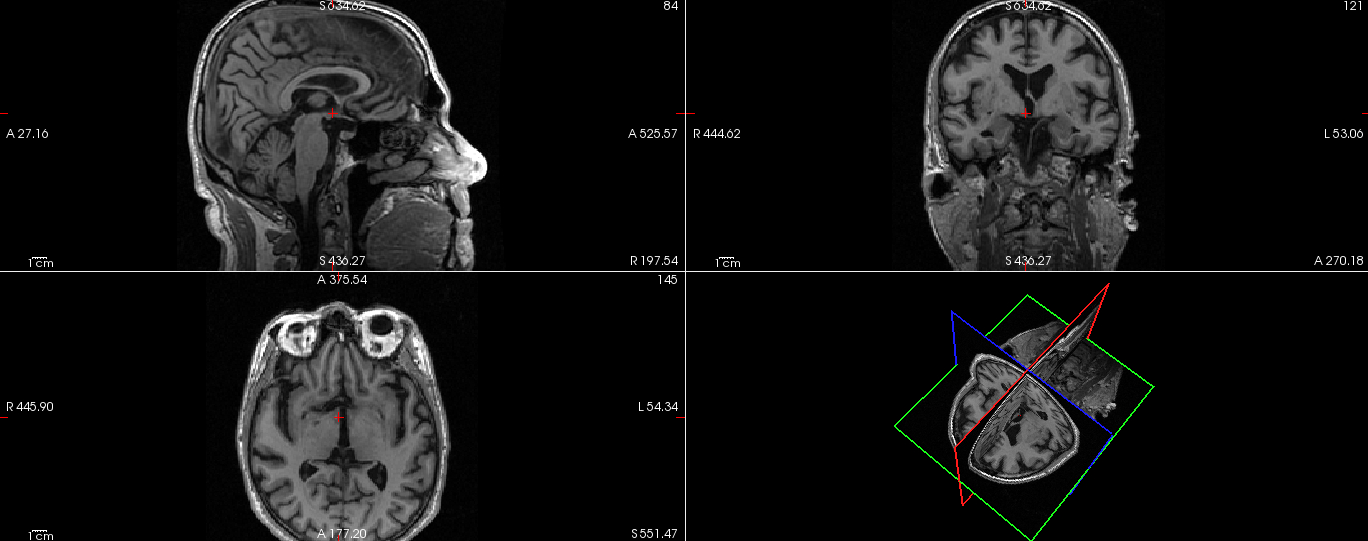
\includegraphics[width=0.95\linewidth]{mymans2}
	\caption{An example of the original image file: \texttt{001.mgz} from subject 002\_S\_0295. This is the original raw image from the MRI-scan and no processing has been done.}
	\label{fig:screenshot001}
\end{figure}



%\begin{figure}
%	\centering
%	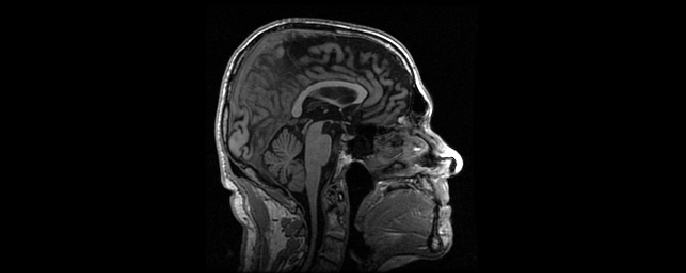
\includegraphics[width=0.7\linewidth]{imgs/mymans_orig_oskar}
%	\caption{}
%	\label{fig:mymansorigoskar}
%\end{figure}


%\begin{table}[H]\label{variable}
%	\centering
%	\begin{tabular}{l l l}
%		\toprule
%		\textbf{Variable} & \textbf{Description} & \textbf{Type} \\ \midrule
%		age & The age of the offenders & Continuous ratio \\
%		priors\_count & The number of previous offences & Discrete interval \\
%		juv\_fel\_count & The number of previous juvenile felonies & Discrete interval \\
%		juv\_misd\_count & The number of previous juvenile misdemeanor & Discrete interval \\
%		c\_charge\_degree & The severity of the offence & Discrete nominal \\
%		race & The race of the offender & Discrete nominal \\
%		age\_cat & The age category of the offender & Discrete nominal \\
%		sex & The sex of the offender & Discrete nominal \\
%		\hdashline
%		score\_text & The COMPAS prediction of chance of recidivism & Discrete interval \\
%		is\_recid & Whether the offender truly recidivated after two years (0/1) & Discrete nominal \\ \bottomrule
%	\end{tabular}
%\end{table} \noindent



\subsubsection{Data Preprocessing}

In this project, the area of interest is the brain itself. 
Therefore, we need to skullstrip the raw images.
The skullstrip process is done by using Freesurfer Software Suite \cite{freesurfer}.
In more depth the skull is removed by using a threshold.
The FreeSurfer software will create files which can be used to check if too much brainmatter is removed in the process of skulstripping the raw image.
Files which can be used to inspect this are: \texttt{brainmask.mgz, T1.mgz, brainmask.gcuts.mgz}

The skulllstripped images are then normalized. 
The images are normalized using \texttt{mri\_normalize}, which converts the white matter image values around 110 \cite{normalize}. %TODO why do we normalize? 
All human brains are different and the raw images are recorded in the subjects personal space. 
In order to compare several brains a registration of the images has to be done to ensure they are all in the same coordinate reference system (CRS). 
A standard CRS for the common brain is called the Tailirach space. 
Each of the raw images in the ADNI-dataset are registered to the Tailirach space using the \texttt{mni305.cor} template from FreeSurfer. 
This is done using \texttt{mri\_vol2vol} which resamples a volume into another field-of-view. 
In this project, a MNI305 transformation has been applied by resampling the original normalized images into talairach space using \texttt{\$subject/mri/transforms/talairach.xfm} %TODO Description of the registration 

\subsubsection{Data Preprocessing Script}




% We use skullstripped 
% We use normalized 
% Template mni305.cor (what does cor stand for)
% what is in the talairach file 
% mri_vol2vol (What does it do) 

% Indtilvidere skriver om advanced registration, talairach space, etc. her


\subsubsection{Data Augmentation}
% Hvis vi vælger at bruge augmentation

\subsection{Explanation of Data Variables}
%subj_id, age, etc. etc. - dette skal findes et sted på server eller ADNI hjemmeside 

\subsection{Visualization of Data}
% Slices of img, preview 
This section aims to give a visulaization of the preprocessed data.


\subsection{Ethicality of Data}
% Quick rant about GDPR

\subsection{Trade off of using fMRI}
%TODO Talk about voxels ( a voxel and encode information about two distinct areas in the brain in same number.see: https://www.youtube.com/watch?v=6wxJ1up-E7E&list=PLIQIswOrUH6_DWy5mJlSfj6AWY0y9iUce )


\section{Methods}
% Short description of all methods
\subsection{Neural Network for Alzheimer's Disease Classification}
In the original Alzheimer's disease classification paper by Camilla, a neural network was used to determine whether each patient had AD. Since this model was full of bias when used on the original data, we used this same model to compare and contrast if the below methods succeeded in removing the most prominent biases from the model. The model was implemented as a PyTorch neural network with 12 convolution layers using ReLU as activation function between each layer. This was followed by a fully connected layer with sigmoid activation to output the probability of each class (sick or healthy). A much more detailed breakthrough of the general project and architecture of the neural network can be seen in \cite{CamillaKandidat}.

\subsection{Model Overview}
%TODO: Hvilke modeller har vi brugt til hvad? Hvor mange cycleGANs har vi trænet?
%TODO: Referér til de forskellige sektioner, hvor man kan finde mere om hver model.

\subsection{Generative Adversarial Network}
Since the meat and potatoes of this project is the cycleGAN, the methods and mathematical understanding behind Generative Adversarial Networks (GANs) will only be briefly explored in this section. A GAN was implemented on the MNIST dataset as a preliminary trail to help understand the basics. This implementation can be seen \href{https://github.com/oskarwiese/AlzPred/blob/main/preliminary/GAN_MNIST.ipynb}{here}. This implementation as well as this section will hopefully help to give the proper insight into the reasoning behind cycleGANs later in this section.

In general, GANs can be seen as two different complex neural networks competing for the best accuracy during  the process of generating a class of pictures. In other words, the networks are adversaries in generating or classifying images, from which the source of the name becomes clear. One of the networks will be focusing on generating a fake version of images seen in a training folder, called the \textit{generator}, and the other will be trying to distinguish between real and fake images, called the \textit{discriminator}. This competition between networks leads to results much better than ever seen in ML and AI image generation, thus making a good foundation for the generation of 1.5T fMRI images from 3T. The two networds are covered in depth in the below subsections.
\begin{figure}[H]
	\centering
	\includegraphics[width=0.7\linewidth]{"imgs/GAN architecture"}
	\caption{The GAN architecture. The generator decodes the random noise from the latent space into a fake image. This fake imgae as well as an image from the training set is fed into the Discriminator, which encodes the data into a binary prediction of whether the image is real or fake.}
	\label{fig:gan-architecture}
\end{figure}


\subsubsection{Generator}


\subsubsection{Discriminator}


\subsubsection{Loss}
For implementing the loss functions necessary to get a proper GAN going, we first need to define some nomenclature. We assume that sample images are sampled from $x \sim p_{\text {data}}(x)$. The discriminator $D(x)$ outputs a value between zero and one determining whether $x$ is real or fake. The generator takes random noise $z \sim p_{\text {data}}(z)$ and returns a fake sample. The loss function for the discriminator is given as shown below.

\[\begin{aligned}
	\mathcal{L}\left(G, D, X, Z\right)_D &=\frac{1}{2} \mathbb{E}_{x \sim p_{x}}[1-D(x)] \\
	&+\frac{1}{2} \mathbb{E}_{z \sim p_{z}}[D(G(z))] \\
\end{aligned}\]
Here, the first term simply forces the discriminator to try to return large values when the samples are real. As the discriminator output approaches 1, the loss approaches 0. The second term is slightly more complicated. The generated image $G(z)$ is given to the discriminator, and the goal of the discriminator is to catch that this is in fact a fake image. Thus, lower discriminator values on the fake image leads to less loss and as the discriminator output approaches 0, this term of the loss also approaches 0.

Now for the generator loss, as we can see below.

\[\mathcal{L}\left(G, D, X, Z\right)_G=-1 \cdot \log \sigma\left(D(G(Z))\right)\]

This loss is equivalent to the BCE loss with logits, where the weights are all set to be equal. The $\sigma$ term is the sigmoid function. This loss function basically states that the generator gets a large loss when the discriminator gets tricked into thinking that the generated image is real. This is due to the fact that a low probability of it being a real image leads to a high loss and vica versa \cite{bcewithlogits}.

\subsection{Specifics}
In this section, other more specific details for the implementation of a GAN will be examined. This includes activation functions, hyperparameters and hyperparameter search and optimizers.

\subsection{CycleGAN}
The GAN allowed for new images in a specific category to be created based on random noise. The next upgrade would be to be able to go from one category to another and back again. This is exactly the problem a cycleGAN aims to fix, which makes it perfect for this paper, since we aim to go from 3T images to 1.5T images. Going back is not as important in this case, but could prove useful for other purposes. The cycleGAN generally works by implementing two generator networks, each generating one category based on an image from the other category, and two discriminator networks, each predicting the probability of the input image actually being from the original category. This architecture is explained and showcased further in figure \ref{fig:cycleganarchitecture} and \ref{fig:cycleganarchitecture2} below.
% TODO: Vigtigt at komme ind på original paper
% F: X -> Y samt G: Y -> X

\subsubsection{General Model Architecture}
% Visualizer library (måske)
\begin{figure}[H]
	\centering
	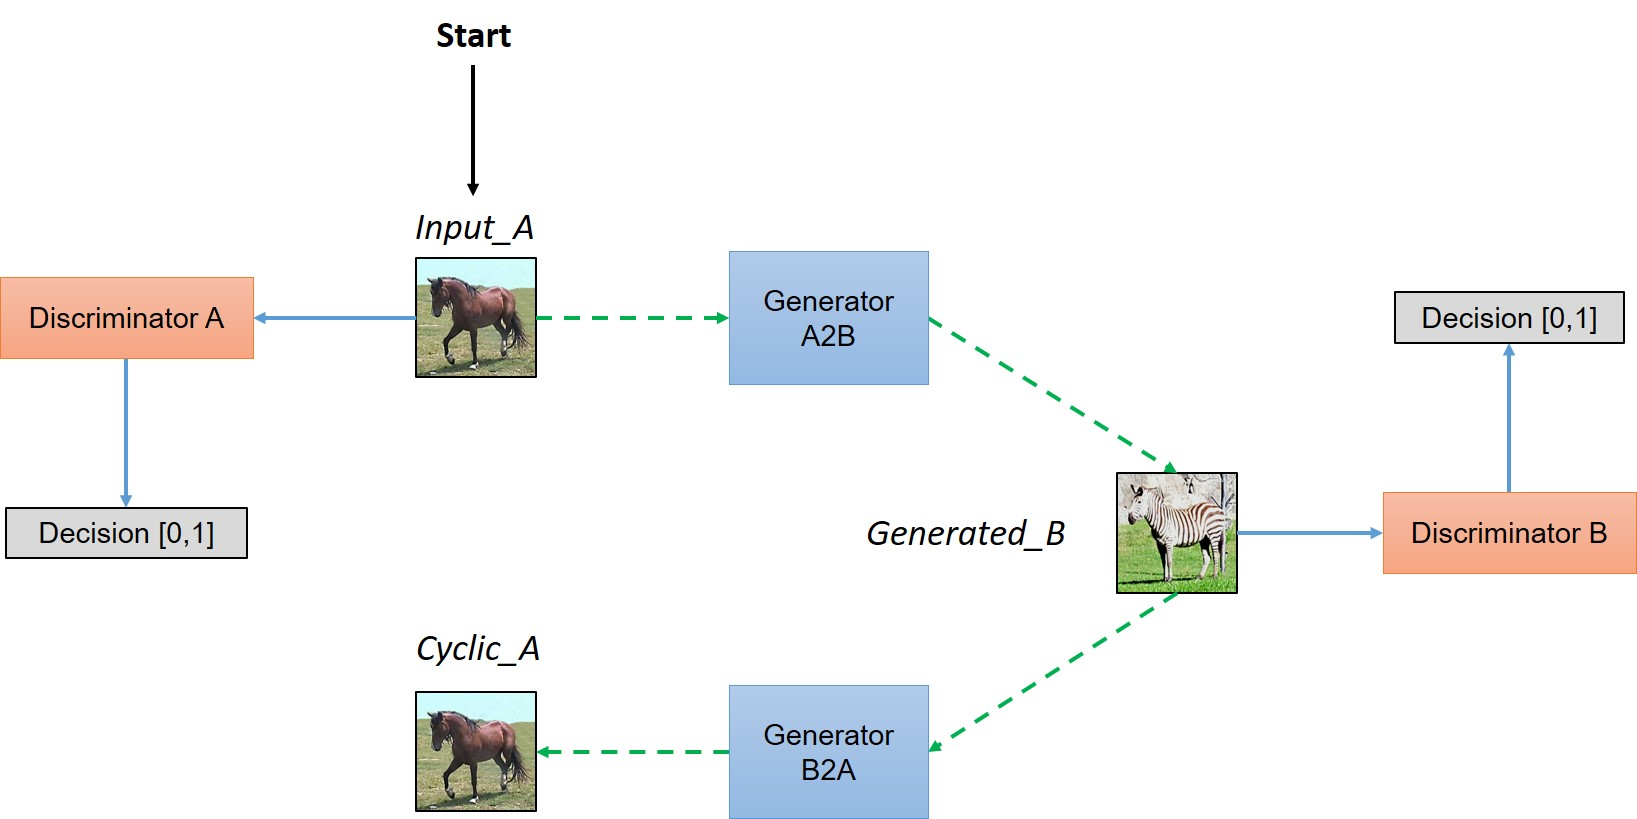
\includegraphics[width=0.7\linewidth]{imgs/cyclegan_architecture}
	\caption{This figure shows the interactions necessary for the four different networks to convert images from A to B. The input image of category A is fed directly to the discriminator and to the generator that converts images from A to B. This generates an attempted image from category B, which is fed both to the discriminator to get a prediction and to the other generator to reconvert the image to one of category A for reasons that will become apparent later in this section.}
	\label{fig:cycleganarchitecture}
\end{figure}

\begin{figure}[H]
	\centering
	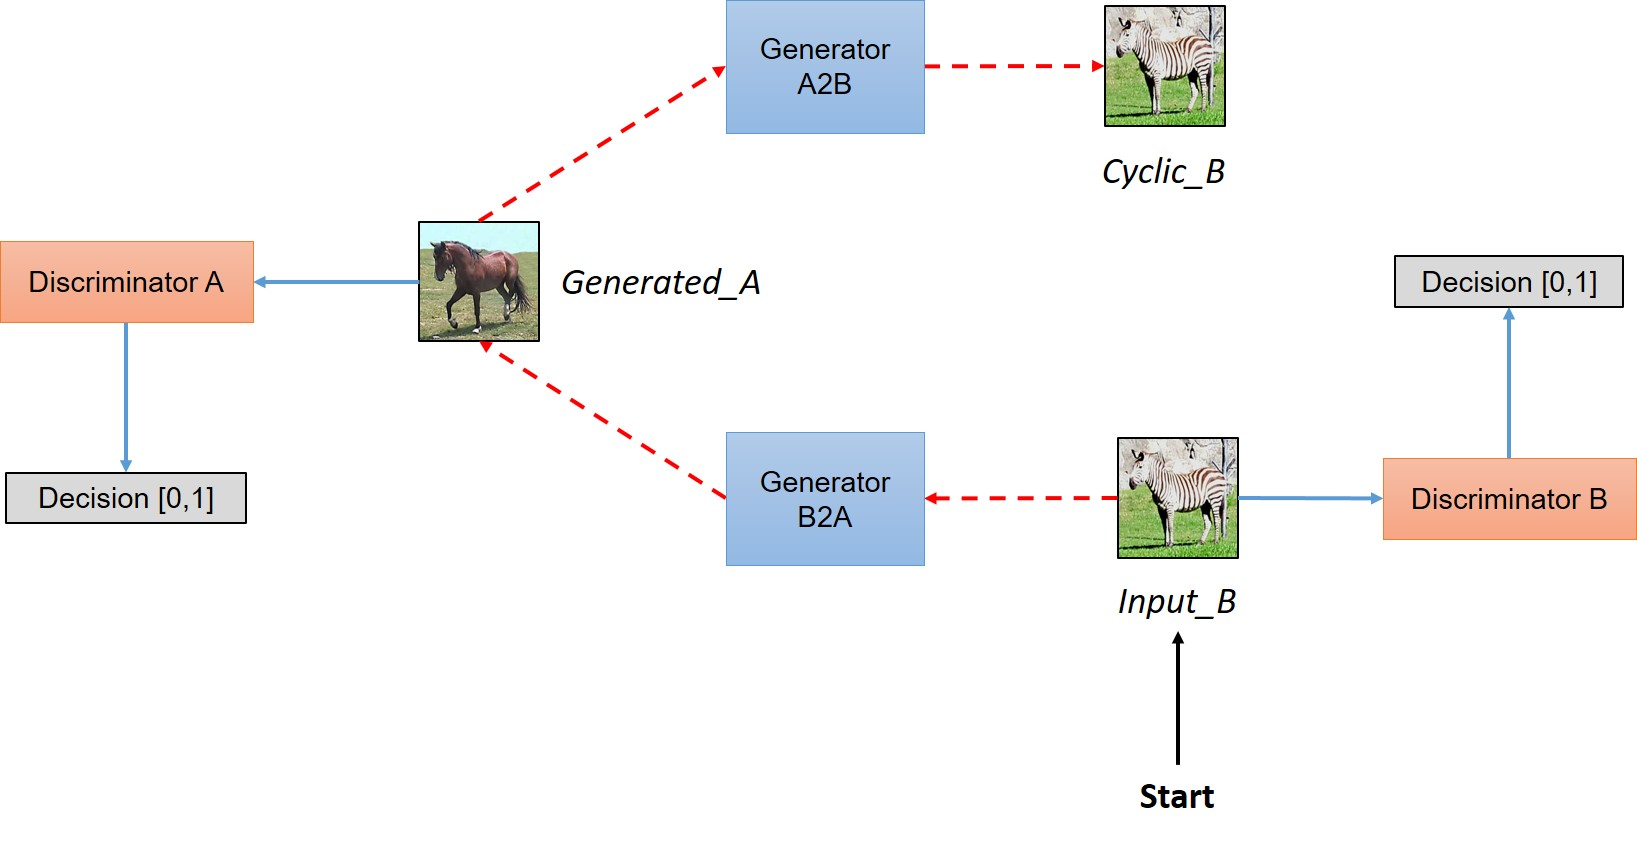
\includegraphics[width=0.7\linewidth]{imgs/cyclegan_architecture2}
	\caption{This figure is almost identical to figure \ref{fig:cycleganarchitecture}, though mirrored in the x and y plane. It shows the interactions necessary for the four different networks to convert images from B to A. For a basic explanation of the components involved, see the caption of figure \ref{fig:cycleganarchitecture}.}
	\label{fig:cycleganarchitecture2}
\end{figure}


\subsubsection{Discriminator in a cycleGAN}
%TODO: Mention the up-sampling structure of the model
The discriminator of the model should take as input an image of size 256x256x1 (since the image is greyscale) and output a prediction of dimension 1x30x30 with values between zero and one. The reason the output is not just one value is because a patch-GAN is used. This move in dimensions is accomplished using up-sampling of the image with 2D-convolutions to extract increasingly abstract features by decreasing the height and width and increasing the depth of the image.

%TODO: Explain the patch-gan structure at the end of the model
To make sure that the model is as robust as possible and to avoid overfitting, a patch-GAN is used before outputting the final image prediction. This works by converting 30x30 blocks of the image into predictions, such that the model is forced to predict the "real-ness" of the image on each of these blocks. This ensures that the discriminator image can accurately predict if the image comes from the generator using any part of the image. Some problems can occur with this method like the model not being about to predict much from a 30x30 square of black pixels. These kinds of problems will be discovered further in the section \ref{discussion} on discussing problems with and efficacies of the model.

%TODO: Explain components (norm and activation layers, convolutions, relu, softmax, prediction layer, etc)
Of just as much importance as the patch-GAN architecture and general model interactions is the layout of each layer and the functions used throughout the discriminator network. A general overview of the layers, kernel size, type of convolution, stride and padding is shown below in figure \ref{fig:cyclegandiscriminatorlayers}.
\begin{figure}[H]
	\centering
	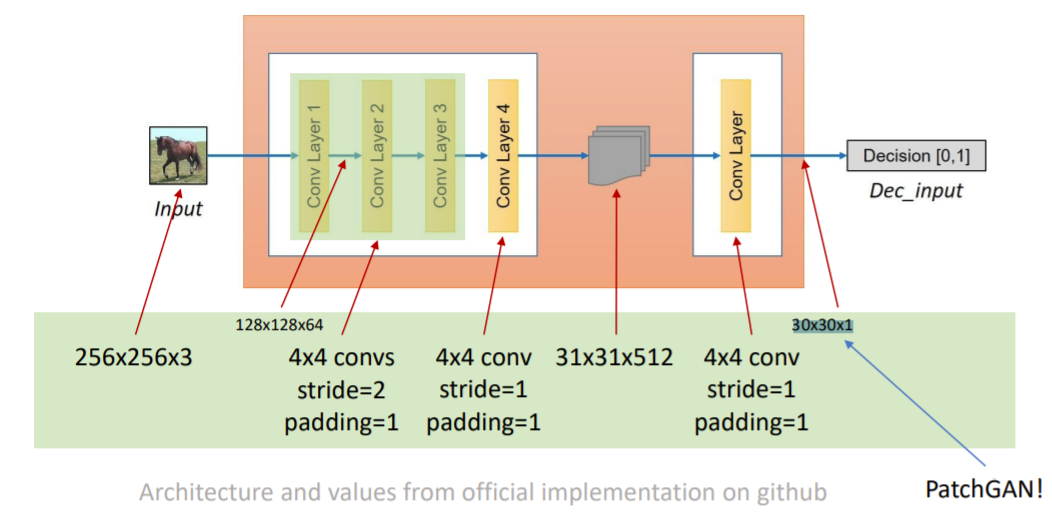
\includegraphics[width=0.7\linewidth]{imgs/cyclegan_discriminator_layers}
	\caption{The primary model layout consisting of the input, layers and output. The input is the grey-scale intensity-based MRI input of size 256x256x1. The five consecutive convolutional layers each have a specified kernel size, stride and padding as noted in the figure. The output is constructed from running the patchGAN on the last layer of the model to get a 30x30x1 matrix of values between 0 and 1. The specific values and layer sizes are specifed in table \ref{discriminator_layers}}
	\label{fig:cyclegandiscriminatorlayers}
\end{figure}

Not shown in the figure is the actions taken between each layer. These include 

\begin{table}[H]\label{discriminator_layers}
	\centering
	\begin{tabular}{lr}\toprule
		Layer                         & Activation Size \\ \midrule
		Input                         & 3x256x256       \\
		64x4x4 conv, stride 2, pad 1  & 64x128x128      \\
		128x4x4 conv, stride 2, pad 1 & 128x64x64       \\
		256x4x4 conv, stride 2, pad 1 & 256x32x32       \\
		512x4x4 conv, stride 1, pad 1 & 512x31x31       \\
		1x4x4 conv, stride 1, pad 1   & 1x30x30         \\ \bottomrule
	\end{tabular}
	\caption{The convolutions, stride and padding of each layer in the discriminators.}
\end{table}

%TODO: Make illustration of actual model layout

\subsubsection{Generator in a cycleGAN}
%TODO: Convolutional neural network
Unlike in a standard GAN generator, where a random image from a latent space is used to create what ends up looking like a real image, the generators in the cycleGAN takes as input an image from one of the datasets. As such, the input dimension is 256x256x1 (since the image is grayscale). The output is of the exact same dimension, since the generator tries to generate an image from the opposite category using the input image. Between input and output, the general generator architecture is that of an autoencoder, as pictured below in figure \ref{fig:autoencoder}. The autoencoder contains three layers in an encoder and a decoder, while 9 so-called resnet blocks reside between them. The encoder encodes features by narrowing the image dimensions down and widening the depth of the data. The decoder does exactly the opposite, using the extracted information to transfer back into the new image. The resnet blocks between the encoder and decoder serve the purpose of interpreting the encoded features. The resnet blocks also use skip connections, which provide an alternate path for the gradient. This helps the network reach convergence.

\begin{figure}[H]
	\centering
	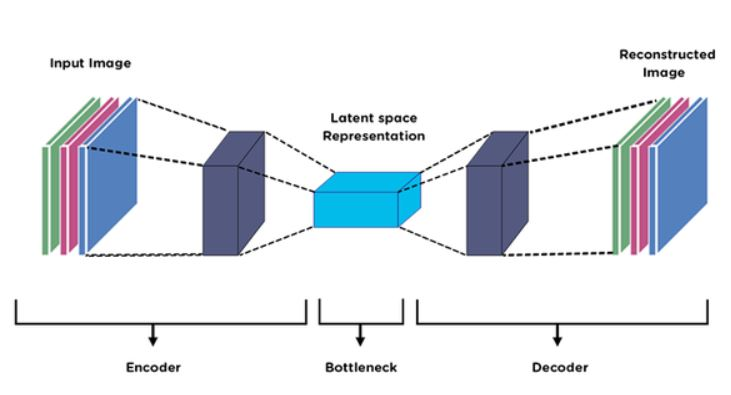
\includegraphics[width=0.7\linewidth]{imgs/autoencoder}
	\caption{The general autoencoder architecture. A kernel does convolutions to reduce and increase the image dimensions. The smaller the dimensions, the larger the feature complexity. The code between the encoder and decoder } %TODO
	\label{fig:autoencoder}
\end{figure}


\begin{figure}[H]
	\centering
	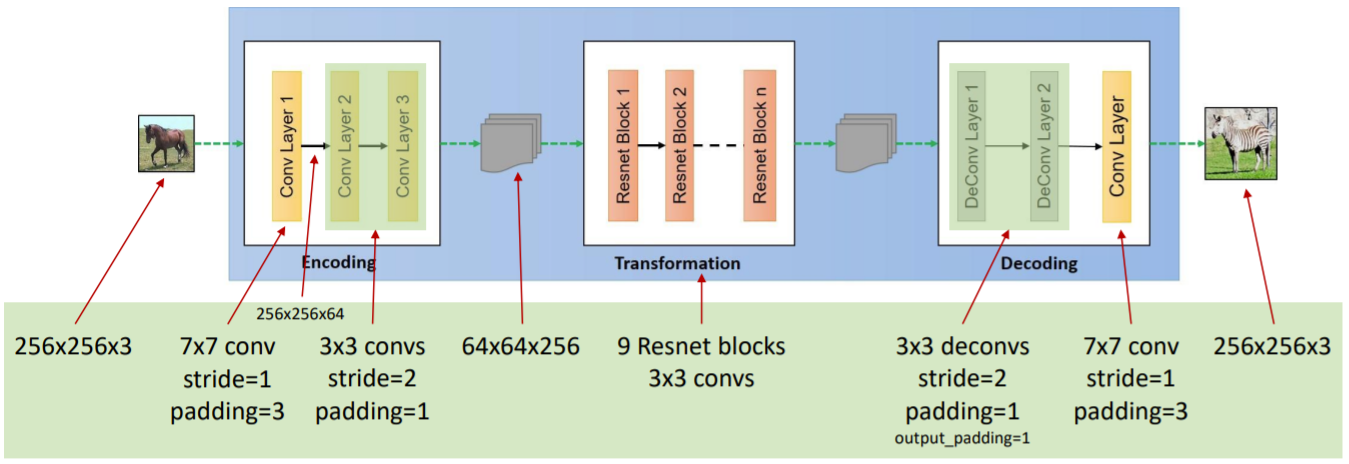
\includegraphics[width=0.7\linewidth]{imgs/cyclegan_generator_layers}
	\caption{The primary model layout consisting of the input, layers and output. The input is the grey-scale intensity-based MRI input of size 256x256x1. The five encoding and decoding convolutional layers as well as the residual blocks each have a specified kernel size, stride and padding as noted in the figure. The specific values and layer sizes are specifed in table \ref{generator_layers}}
	\label{fig:cyclegangeneratorlayers}
\end{figure}


%TODO: Explain components (norm and activation layers, convolutions, relu etc)
\begin{table}[H]\label{generator_layers}
	\centering
	\begin{tabular}{lr}\toprule
		Layer                                            & Activation Size \\ \midrule
		Input                                            & 3x256x256       \\
		64x7x7 conv, stride 1, pad 3                     & 64x256x256      \\
		128x3x3 conv, stride 2, pad 1                    & 128x128x128     \\
		256x3x3 conv, stride 2, pad 1                    & 256x64x64       \\
		9 residual blocks                                & 256x64x64       \\
		128x3x3 convTranspose, stride 2, pad 1, outpad 1 & 128x128x128     \\
		64x3x3 convTranspose, stride 2, pad 1, outpad 1  & 64x256x256      \\
		3x7x7 conv, stride 1, pad 3                      & 3x256x256       \\ \bottomrule
	\end{tabular}
	\caption{The convolutions, stride and padding of each layer in the generators.}
\end{table}

%TODO: Make illustration of actual model layout

\subsubsection{Objective Functions (Losses)}
For this section, a number of notations will be introduced. Since the goal is to map between the two domains $X$ and $Y$, we introduce $G : X \rightarrow Y$ and $F : Y \rightarrow X$. Furthermore, $y \sim p_{\text {data}}(y)$ and $x \sim p_{\text {data }}(x)$ refer to the distributions of each domain and $x$ and $y$ refer to samples from each domain. Lastly, the discriminators for each domain are given by $D_X$ and $D_Y$.

This section will focus on how the objective functions are constructed to ensure the correct result from the discriminators and generators. In general, the losses are separated into three categories: adversarial losses, cycle-consistency losses and identity losses. 

Here, the adversarial losses aim to ensure that discriminators are able to distinguish between real and fake images and generators are able to generate convincing fake images, the cycle-consistency losses make sure that mapping an image through the two different generators one after the other will result in approximately the same image as in the beginning and the identity losses check that the generators do not augment images that are already part of the domain they map towards. More details on each of these losses can be seen in the rest of this subsection.

When added together, the final cost function will look as shown below.

%TODO: The full loss (objective)
Our full objective is:
\[\begin{aligned}
	\mathcal{L}\left(G, F, D_{X}, D_{Y}\right) &=\mathcal{L}_{\mathrm{GAN}}\left(G, D_{Y}, X, Y\right) \\
	&+\mathcal{L}_{\mathrm{GAN}}\left(F, D_{X}, Y, X\right) \\
	&+\lambda_{cyc} \mathcal{L}_{\mathrm{cyc}}(G, F) \\
	&+\lambda_{iden} \mathcal{L}_{\mathrm{iden}}(G, F)
\end{aligned}\]

\noindent Here, $\mathcal{L}_{\mathrm{GAN}}\left(G, D_{Y}, X, Y\right)$ and $\mathcal{L}_{\mathrm{GAN}}\left(F, D_{X}, Y, X\right)$ are the adversarial losses for $G$ and $D_Y$ and $F$ and $D_X$ respectively. Meanwhile, $\mathcal{L}_{\mathrm{cyc}}(G, F)$ is the cyclic loss for both generators and $\mathcal{L}_{\mathrm{iden}}(G, F)$ is the identity loss for both generators. The values $\lambda_{cyc}$ and $\lambda_{iden}$ are hyperparameter weights, controlling the respective importance of each part of the total loss function.

The goal of the final loss function is now to have the generators $G$ and $F$ minimize the function and have the discriminators $D_X$ and $D_Y$ maximize the function. This leads to competition between the four models. This interplay can be seen below.

\begin{equation}\label{minimax}
	G^{*}, F^{*}=\arg \min _{G, F} \max _{D_{x}, D_{Y}} \mathcal{L}\left(G, F, D_{X}, D_{Y}\right).
\end{equation}

%TODO: Discriminator and generator adversarial loss
The adversarial losses are principally the simplest of the losses to understand. They simply make sure that the discriminators are very sure that real images are real and fake images are fake, while the generator becomes increasingly better at fooling the discriminator (creating convincing fake images). Modeling this behavior into an equation is simple, since the discriminator $D_Y$ approaches minimal adversarial loss as it gets closer to predicting 1 for real images and 0 for generated images. Meanwhile, the opposite is true for the generator. Since the discriminators want to maximize the below equations and the generators want to minimize them, these models have an antagonistic relationship and constantly need to sacrifice the performance of the other model to get better performance itself. This has been shown countless times in the literature to be fruitful and is the basis of GAN-based techniques.

\[\begin{aligned}
	\mathcal{L}_{\mathrm{GAN}}\left(G, D_{Y}, X, Y\right) &=\mathbb{E}_{y \sim p_{\text {data }}(y)}\left[\log D_{Y}(y)\right] \\
	&+\mathbb{E}_{x \sim p_{\text {data }}(x)}\left[\log \left(1-D_{Y}(G(x))\right],\right.
\end{aligned}\]

\[\begin{aligned}
	\mathcal{L}_{\mathrm{GAN}}\left(F, D_{X}, X, Y\right) &=\mathbb{E}_{x \sim p_{\text {data }}(x)}\left[\log D_{X}(x)\right] \\
	&+\mathbb{E}_{y \sim p_{\text {data }}(y)}\left[\log \left(1-D_{X}(F(y))\right],\right.
\end{aligned}\]

%TODO: Forward and backward consistency loss
It turns out that the above adversarial losses are not always strenuous enough to map the input $x_i$ to an output $y_i$. Therefore, another set of loss functions are added; the forward and backward consistency loss functions. The goal of these functions is to make sure that an image from $X$ mapped to $Y$ and mapped back to $X$ again will closely resemble the original image. That is, $x \rightarrow G(x) \rightarrow F(G(x)) \approx x$.This concept is called forward cycle consistency loss, while the same is true for the other direction, backward cycle consistency loss: $y \rightarrow F(y) \rightarrow G(F(y)) \approx y$. As can be seen in the two equations below, the L1-loss is taken between the original image $x$ and the double-generated image $F(G(x))$. The generators $G$ and $F$ then aim to minimize these terms, such that the two images are as closely resembling as possible. This loss is focused on the generators specifically, since the discriminators only play a roll in predicting if the image is real.

\[\begin{aligned}
	\mathcal{L}_{\text {cyc }}(G, F) &=\mathbb{E}_{x \sim p_{\text {data }}(x)}\left[\|F(G(x))-x\|_{1}\right] \\
	&+\mathbb{E}_{y \sim p_{\text {dau }}(y)}\left[\|G(F(y))-y\|_{1}\right] .
\end{aligned}\]

%TODO: Identity loss
The identity loss punishes the model if the generator changes an image that is already part of the domain it transforms to. That is, $y_{new} = G(y)$ gets zero identity loss if $y_{new}$ and $y$ are completely identical and high loss if there are vast differences. The identity loss usually keeps the generators from changing the colors of the input image to get lower errors. The identity loss has therefore not been used in out implementation, as we are not working with color images. The loss has been included for completeness and for possible inspiration if color images were to be used in other contexts.

\[\begin{aligned}
	\mathcal{L}_{\text {iden }}(G, F) &=\mathbb{E}_{x \sim p_{\text {data }}(x)}\left[\|F(y)-x\|_{1}\right] \\
	&+\mathbb{E}_{y \sim p_{\text {data }}(y)}\left[\|G(x)-y\|_{1}\right] .
\end{aligned}\]


\subsubsection{optimizer, cross Entropy, Etc.}
A table of the used hyperparameters and their values in this project in given below. Note that these hyperparameters are applied to different models. Kernel size, stride and padding for each of the convolutional layers of the discriminator and generator are shown in table %TODO: Lav tabel over kernel size, stride og padding.

	\begin{table}[H]
	\centering
	\begin{tabular}{l l l l l l l l l}
		\toprule
		& \textbf{Hyperparameter}           &&&&& & \textbf{Value}   & \\ \midrule
		& \multicolumn{7}{c}{\textbf{General}}          & \\
		& Batch size              &&&&& & $1$           & \\
		& Learning rate [$\alpha$]&&&&& & $1e-5$        & \\
		& $\lambda_{iden}$        &&&&& & $0$           & \\
		& $\lambda_{cyc}$         &&&&& & $10$          & \\
		%& Number of workers      &&&&& & $4$           & \\
		& Number of epochs        &&&&& & $10$          & \\
		& Betas                   &&&&& & $(0.5, 0.999)$& \\
		& \multicolumn{7}{c}{\textbf{Discriminator}}    & \\
		& input dimension         &&&&& & $1x256x256$   & \\
		& Conv depths             &&&&& & $\left[3, 64, 128, 256, 512\right]$& \\
		& Output dimension        &&&&& & $1x30x30$     & \\
		& Leaky-ReLU activation   &&&&& & $0.2$         & \\
		& \multicolumn{7}{c}{\textbf{Generator}}        & \\
		& Input dimension         &&&&& & $1x256x256$   & \\
		& Conv depths             &&&&& & $\left[64, 128, 256, 128, 64\right]$              & \\
		& Output dimension        &&&&& & $1x256x256$   & \\ \bottomrule
		%& Train-test split         &&&&& & $0.8/0.2$& \\
	\end{tabular}
\end{table} 
The batch size, learning rate, $\lambda_{cyc}$ and betas were set to the same value as in the original CycleGAN paper, as this turned out to be efficacious on ADNI images too. Most notably, the number of epochs has been drastically reduced (from 200 in the original paper to 10). This is due to the fact that the training data used in this project is much more plentiful than originally used to train the first CycleGAN in the paper. This means that we can get away with using vastly fewer epochs. The weight $\lambda_{iden}$ was set to zero in this paper. This is because RGB images have not been used in this project and color integrity is therefore not important in the generator output.

The discriminator and generator convolution depths were chosen to match those used in the original CycleGAN paper. It is self-explanatory that using other images (RGB, non-square, different dimension) would require changing the architecture of input and output dimensions of all four models while also ensuring that the kernel size, stride and padding of the convolutional layers are setup correctly. This can be double checked by using $output\_dim = n - k + p + 1$, where $n$ is the image dimension, $k$ is kernel size and $p$ is padding.

\subsubsection{Troubleshooting}\label{troubleshooting}%TODO: Skal måske faktisk stå i results???
% Image Issues
Since implementing a cycleGAN requires implementing four different neural networks, the hyperparameter search and minutia of the model can be difficult to get right. Very many issues like non-convergence, mode collapse, diminished gradients, vanishing gradients and more are well documented \cite{hard_to_train}. A known problem is cycleGAN only training until they reach a local minimum \cite{ganlocalminimum}. Another is the issue of getting noisy black and white squares in black-and-white images, sometimes referred to as checkerboard noise. One of the first models that was trained on the MRI ADNI images turned out to contain a version of this checkerboard noise. The source of the noise turned out to be an uneven sampling of pixels in earlier layers to newer layers when doing the upsampling (also known as transpose convolution or deconvolution). Mismatches between the kernel size and the stride as well as bad upscaling can cause some areas of the upsampled image to contain information from more pixels than others. This is a critical cause of the recognizable checkerboard noise \cite{checkerboard}. An illustration of how the flaw gets made can be seen below. images generated from the flawed cycleGAN can also be seen in illustration \ref{fig:troubleshoota}. Here, it is clear that white squares are surrounded by black squares all over the image, worsening the general image quality.

\begin{figure}[H]
	\centering
	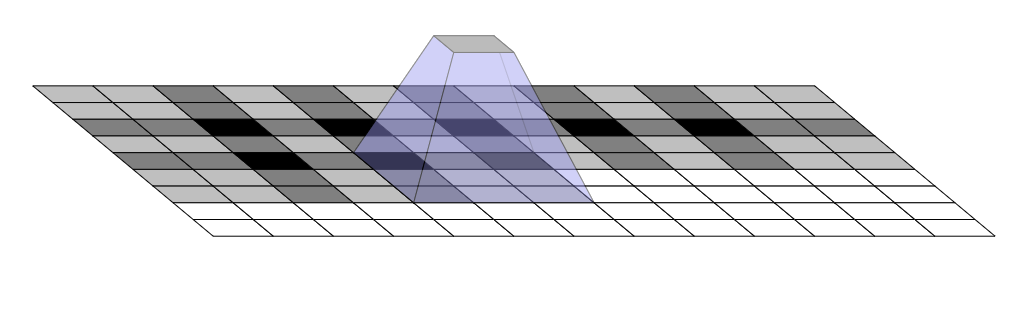
\includegraphics[width=0.7\linewidth]{imgs/deconvolution_mismatch}
	\caption{When the kernel size is not divisible by the stride, the image gets higher intensity in some areas than others leading to a checkerboard pattern. Shown here is a deconvolution using kernel size of 3 and stride of 2. Figure courtesy of \cite{checkerboard}.}
	\label{fig:deconvolutionmismatch}
\end{figure}
Solving this problem in practice first required separating upsampling from convolution. This works since the more intensity between pixels is split between multiple pixels. Doing this in practice involved switching every deconvolution layer except the last one from \texttt{nn.ConvTranspose2d(in\_channels, out\_channels, **kwargs)} to first \texttt{nn.Upsample(scale\_factor=2, mode='bilinear', align\_corners=True)} and then \texttt{nn.Conv2d(in\_channels, out\_channels, **kwargs)}. In a nutshell, instead of running a transpose convolution, an upsampling is perform to double the size of the image using bilinear interpolation and then a standard convolution is performed. This not only solves most of the checkerboard issues but also ensures that the model is able to learn from the decoding, since (\texttt{nn.Conv2d} and \texttt{nn.ConvTranspose2d} have trainable kernels while \texttt{nn.Upsample} does not) \cite{learnableKernel}. After implementing this functionality, the generated images now look like shown in illustration \ref{fig:troubleshootb}. We now see that most of the checkerboard artifacts are gone, though some vertical and horizontal lines still persist. A weird white void has also been generated around about half of the images for some reason.

The slight lines in the generated images after using bilinear interpolation for upsampling are not nearly as problematic but are still unfortunate as a final output. To solve this, we implemented a kernel size that was divisible by the stride in the deconvolution layers, as mentioned in the previous paragraph. This should make the kernel spread information from each pixel more evenly between new pixels and supply a less grainy final image \cite{checkerboard}. In illustration \ref{fig:troubleshootc}, most of the noise has finally been removed and no lines persist in the image. The white voids around the brain seems to have become even more prevalent though, which also needs to be fixed. This was taken care of by replacing bilinear interpolation with nearest-neighbor interpolation. The result of replacing the interpolation can be seen in \ref{fig:troubleshootd}. It is now evident that basically no noise is left in the image, and most of the troubleshooting relating to image quality has thus subsided. The full comparison between results after each improvement has been implemented, can be seen in figure \ref{fig:troubleshoot}.

\begin{figure}[H]
	\centering
	\begin{subfigure}[b]{0.7\textwidth}
		\centering
		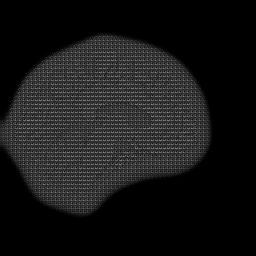
\includegraphics[width=0.475\linewidth]{imgs/1.5T_MRI_artifact}%
		\hfill
		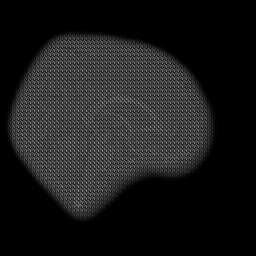
\includegraphics[width=0.475\linewidth]{imgs/3T_MRI_artifact}
		\caption{1.5T and 3T respectively YZ MRI images from the preliminary run.}
		\label{fig:troubleshoota}
	\end{subfigure}
	\vskip\baselineskip
	\begin{subfigure}[b]{0.7\textwidth}
		\centering
		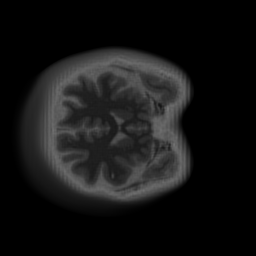
\includegraphics[width=0.475\linewidth]{imgs/vertical_noise_example}%
		\hfill
		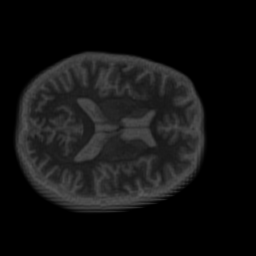
\includegraphics[width=0.475\linewidth]{imgs/horizontal_noise_example}
		\caption{1.5T and 3T respectively YZ MRI images after bilinear interpolation has been implemented in upsampling.}
		\label{fig:troubleshootb}
	\end{subfigure}
	\vskip\baselineskip
\end{figure}
\begin{figure}[H]
	\centering
	\begin{subfigure}[b]{0.7\textwidth}
		\centering
		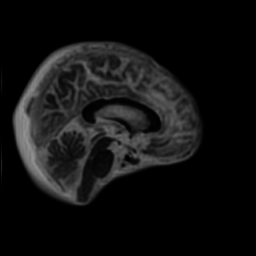
\includegraphics[width=0.475\linewidth]{imgs/1.5T_bilinear}%
		\hfill
		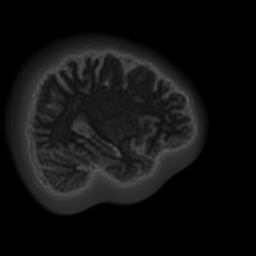
\includegraphics[width=0.475\linewidth]{imgs/3T_bilinear}
		\caption{1.5T and 3T respectively YZ MRI images after making kernel size divisible by stride.}
		\label{fig:troubleshootc}
	\end{subfigure}
	\begin{subfigure}[b]{0.7\textwidth}
		\centering
		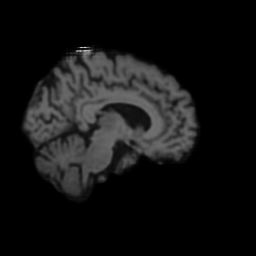
\includegraphics[width=0.475\linewidth]{imgs/1.5T_no_noise}
		\hfill
		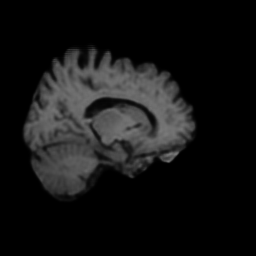
\includegraphics[width=0.475\linewidth]{imgs/3T_no_noise}
		\caption{1.5T and 3T respectively YZ MRI images after bilinear interpolation has been changed to nearest neighbor interpolation.}
		\label{fig:troubleshootd}
	\end{subfigure}
	\caption{Comparison of troubleshooting efforts to solve the visual issues in the generated images from the generators.}
	\label{fig:troubleshoot}
\end{figure}
Even after the struggle of implementing all of the these changes, some challenges are still present when generating images, though at this point the severity of the problems has been significantly reduced. It turns out that images that are converted from $3T$ to $1.5T$ get a coupe horizontal white lines in the top of the image. This artifact can be seen in figure \ref{fig:troubleshoot_horizontals} for a random subject for each field-strength, where the above explained case manifested itself.

\begin{figure}[H]
	\centering
	\begin{subfigure}[b]{0.7\textwidth}
		\centering
		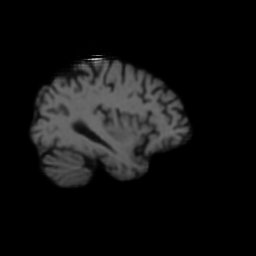
\includegraphics[width=0.475\linewidth]{imgs/1.5T_hori1}%
		\hfill
		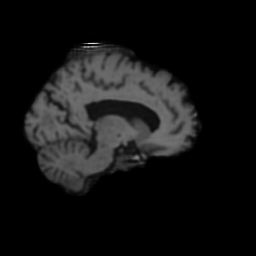
\includegraphics[width=0.475\linewidth]{imgs/1.5T_hori2}
	\end{subfigure}
	\caption{Two generated images before training was completed (half an epoch and one and a half epochs respectively). The left image is 1.5T and the right is 3T. The image artifact occurs only on the top of the $1.5T$ images, where a trading pattern of low-intensity and high-intensity pixels can be seen forming small horizontal lines.}
	\label{fig:troubleshoot_horizontals}
\end{figure}
Since this problem seems to exist in such a small part of the images, it has been decided that resolving this issue will be left as future work. For future reference, the problem likely transpires because the combination of kernel size and stride is still not completely optimized. This means that especially areas varying between low- and high-intensity pixels will be less refined than other areas of the image. Why this error only happens at the top of the image is, for the time being, a mystery.
\\\\
% Mode Collapse
Another issue entirely turned out to be that the vast number of input images all mapped to the same output image. This problem is well-known and is commonly called mode collapse. Figuring out that the models suffered from mode collapse normally required either plotting loss curves and seeing oscillations in the generator loss or sampling a number of images using different input images. In the generator models from this paper, no signs of mode collapse could be seen in the loss curves except for the discriminator constantly having very low loss. It was very evident that the generator only created one image when given multiple input images though \cite{mode_collapse_MLM}. Examples of the images used to test for mode collapse and the resulting generator output images are shown below in figure \ref{label}.

%TODO: få billeder fra mode collapse
%\begin{figure}
%	
%\end{figure}
Many solution to the problem of mode collapse exist, some being much easier to implement than other. Easier solutions include reducing the learning rate, making separate learning rates for the discriminators and generators and only updating the discriminator if the accuracy of the discriminator in the current step is under 50\%. Harder solutions include implementing instance noise, making the generator better or making the discriminator worse. For the discriminators in this project, it turned out that it was enough to implement the accuracy check before updating the discriminators, reducing the learning rate and making separate learning rates for generators and discriminators. The others methods have been left in this section for future reference \cite{mode_collapse_reddit_fix}\cite{mode_collapse_github}. After implementing these fixes, the model was able to generate output samples from a much larger distribution, which indicates that the mode collapse has been fixed. A number of generated images can be seen in section \ref{results}.

\subsubsection{Classifier}


\subsection{Reproducibility}\label{repro}
This section aims to give the reader a precise insight into how the methods of this project were implemented and how it would be possible to reproduce these results in the future. Hopefully, this will also simplify the methods. Reproducibility is an important part of writing any project or performing any research. It shows significance of the given result if it is possible for others at a later time to replicate or reproduce the results, since it validates the result of the original study and shows that it was not a fluke. All of the code is written in Python Version 3.9 and PyTorch version a%TODO find version. Gælder også de tre pakker i tabellen nedenfor
Furthermore, the versions of the packages used in the project are given in the table below. If running any code from this project, please make sure that your packages either as new or newer than the ones specified below. All code for the project is accessible at \url{https://github.com/oskarwiese/AlzPred/tree/main/oskar_implemetation}.
\begin{table}[H]
	\begin{center}
		\begin{tabular}{l l l l l l l l l l}
			\toprule
			& \textbf{Package}      & & & & & & & \textbf{Version}  & \\ \midrule
			& torchvision   & & & & & & & $0.10.0$ & \\
			& pelutils      & & & & & & & $0.6.9$  & \\
			& torch         & & & & & & & $1.9.0$  & \\
			& tqdm          & & & & & & & $4.62.3$ & \\
			& numpy         & & & & & & & $1.21.2$ & \\
			& matplotlib    & & & & & & & $3.4.3$  & \\
			& random        & & & & & & & $a$      & \\
			& os            & & & & & & & $a$      & \\
			& PIL           & & & & & & & $a$      & \\
			& albumentations& & & & & & & $1.1.0$  & \\ \bottomrule
		\end{tabular}
	\end{center}
\end{table}
\noindent Since randomness plays a large roll in implementing deep learning architectures, random seeds have been set in order to ensure equivalent results for every run of the notebook. The seed number was set to 42 and was used for the python seed \texttt{random.seed}, the numpy seed \texttt{np.random.seed} and the pytorch seeds \texttt{torch.manual\_seed} \texttt{torch.cuda.manual\_seed}
\texttt{torch.cuda.manual\_seed\_all} and were set before any processes were run in any of the scrips used.

In order to make the results as reproducible as possible, the data as well as the way the data was obtained also plays a big role. The way the data was obtained can be seen described in full detail in section \ref{dataDescription}. The data originally comes from the ADNI studies, but the data used specifically for this project was the folders \texttt{/dtu-compute/ADNIbias/freesurfer\_ADNI1} and \texttt{/dtu-compute/ADNIbias/freesurfer\_ADNI2} on the DTU HPC server.\\

\begin{table}[H]\label{fig:files}
	\begin{center}
		\begin{tabular}{l l l l l l l l l}
			\toprule
			& \textbf{File}          & & & & & & \textbf{Description}  & \\ \midrule
			& train.py               & & & & & & \makecell[tl]{Main script which runs the training loop \\ and saves the final models} & \\
			& discriminator\_model.py& & & & & & Definition of the discriminator architecture & \\
			& generator\_model.py    & & & & & & Definition of the generator architecture & \\
			& utils.py               & & & & & & \makecell[tl]{Utility functions like plotting, save/load \\ checkpoint and seeding} & \\
			& dataset.py             & & & & & & Preprocessing of the dataset & \\
			& config.py              & & & & & & Paths and hyperparameter definition & \\ \bottomrule
		\end{tabular}
	\end{center}
\end{table}

\noindent Below, a thorough walkthrough of the most essential parts of the code will be made. The code is split between six different files, the names and short descriptions of which can be seen in table \ref{fig:files}. 

The primary file is \texttt{train.py}, which is responsible for putting all of the functionality together. This script starts by defining each of the four models (generators/discriminators) as well as the optimizers and losses. Afterwards, it loads in the dataset and starts the training loop. This loop calls the function \texttt{train\_cykel} where all model interactions and singular losses are immediately calculated. Afterwards, adversarial loss, cycle-consistency loss and identity loss are found and added to get the final loss. This loss is then backpropagated through the model and the next batch is run.

The next two files, \texttt{discriminator\_model.py} and \texttt{generator\_model.py} are related in the sense that they both define the general functionality of models used in \texttt{train.py}. In \texttt{discriminator\_model.py}, the \texttt{Block} class defines the architecture of using one convolution and applying instance normalization and leaky-ReLU, which becomes useful often. The class \texttt{Discriminator} is the workhorse of the script. This class initially defines a layers applying a 2D convolution and leaky-ReLU, after which a number of blocks are added. At the end of the architecture, a last convolutional layer is added and sigmoid is applied to output probabilities. In the script \texttt{generator\_model.py}, the \texttt{ConvBlock} class defines a convolution consisting of a 2D convolution, instance normalization and applying ReLU. The \texttt{ResidualBlock} class consists of two \texttt{ConvBlock} calls. Both of these classes help to implement the general architecture in the \texttt{Generator} class. The \texttt{Generator} class has an initializer made up of an initial layer, down-blocks, up-blocks, residual blocks and a last layer. These are called in the forward method, where an initial layer is first added, then the down-blocks, the residual blocks, the up-blocks and at last the final layer. On top of this, tan-h is applied to the model output.

The script \texttt{config.py} is very short but extremely important for the general workflow and successful use of the code. It defines the directories of the data and almost all hyperparameters that might need to be changed at any point for any reason when running the code.

The script \texttt{utils.py} and \texttt{dataset.py} are not as important to the general workflow and are much easier to understand. \texttt{utils.py} simply implements functions that save and load a checkpoint (current model and optimizer states) such that training can easily be stopped or the best model can be saved. Functions are also saved to plot the loss curves and add seeds to everything, so randomness does not provide difficulty. \texttt{dataset.py} does all the data preprocessing.

\section{Results}\label{results}
%TODO: Hvordan vurderer vi, hvor godt vi har klaret os?
%TODO: Indsæt de bedste genererede billeder fra 1.5T og 3T
%TODO: Indsæt loss-kurve
%TODO: Undersøg (og lav eventuelt grafer for) hvor ofte discriminatoren får ret i ægte/falske billeder
%TODO: Måske også en graf for hvor ofte generatoren snyder discriminatoren?
%TODO: Prøv at generere billeder fra alle tre orienteringer og se, om de bliver genereret lige effektivt
%TODO: Sammenlign valideringsbilleder med genererede billeder og brug metrics til at måle forskellen mellem billederne
%TODO: Hvor godt klarer modellen sig når man afprøver cycle consistency? Hvor meget bliver billedet ændret, hvis man giver 1.5T->3T modellen et 3T-billede?
%TODO: https://machinelearningmastery.com/how-to-evaluate-generative-adversarial-networks/
%Once your confidence in developing GAN models improves, both the Inception Score and the Frechet Inception Distance can be used to quantitatively summarize the quality of generated images. There is no single best and agreed upon measure, although, these two measures come close.

This section will focus on showing relevant outputs of the final trained models. Results from previous, less successful models can be found in section \ref{appendix} and section \ref{troubleshooting} highlights some of largest issues during the image generation and how they were solved. The general goal of this section will be to first go through examples of generated images and compare and contrast them to real images, and secondly to show loss-curves for each model. Sections \ref{xy_generated}, \ref{xz_generated} and \ref{yz_generated} provide examples of generated images from the models trained on the $XY$, $XZ$ and $YZ$ respectively. In a slightly different manner, section \ref{training_progress} shows how training comes along after a number of steps to show what the generators learn and when. Afterwards, section \ref{all_generated} will show results on every plane when a model has been trained on data from all of $XY$, $XZ$ and $YZ$. Afterwards, the next four sections will focus on the various losses. The sections \ref{disc_loss}, \ref{gen_loss}, \ref{cycle_loss} and \ref{iden_loss} will show respectively the discriminator losses, generator losses, cycle losses and identity losses from each of the four aforementioned models.

\subsection{Training Progress}\label{training_progress}
%TODO: Fyld ud med de rigtige billeder og skriv figurtekst
\begin{figure}[H]
	\centering
	\begin{subfigure}[b]{0.7\textwidth}
		\centering
		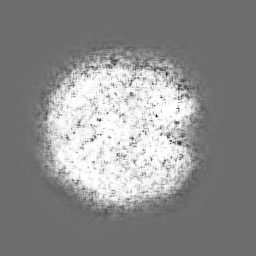
\includegraphics[width=0.32\linewidth]{imgs/placeholder_idx_0}
		\hskip\skipper
		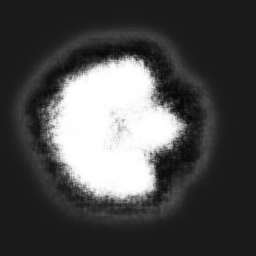
\includegraphics[width=0.32\linewidth]{imgs/placeholder_idx_4000}
		\hskip\skipper
		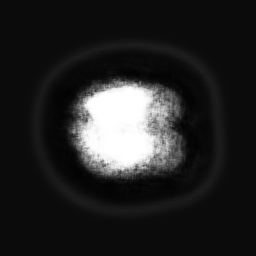
\includegraphics[width=0.32\linewidth]{imgs/placeholder_idx_10000}
	\end{subfigure}
	\vskip\ripper
	\begin{subfigure}[b]{0.7\textwidth}
		\centering
		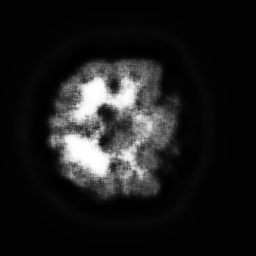
\includegraphics[width=0.32\linewidth]{imgs/placeholder_idx_14000}
		\hskip\skipper
		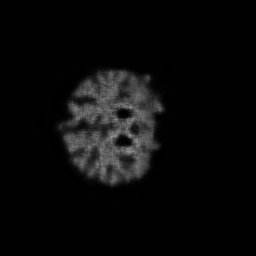
\includegraphics[width=0.32\linewidth]{imgs/placeholder_idx_25000}
		\hskip\skipper
		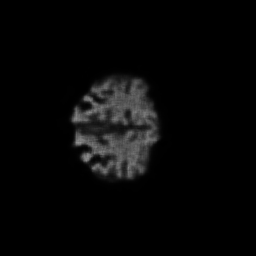
\includegraphics[width=0.32\linewidth]{imgs/placeholder_idx_40000}
	\end{subfigure}
%	\caption{1.5T and 3T respectively YZ MRI images after bilinear interpolation has been changed to nearest neighbor interpolation.}
%	\label{fig:troubleshootd}
\end{figure}

\subsection{XY Generated Images}\label{xy_generated}
%TODO: Fyld ud med de rigtige billeder og skriv figurtekst
%TODO: Her er tanken at rows eller columns indeholder ægte 3T, ægte 1.5T, reconstructed 3T og reconstructed 1.5T
\begin{figure}[H]
	\centering
	\begin{subfigure}[b]{0.7\textwidth}
		\centering
		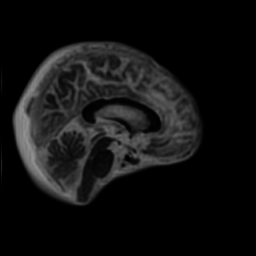
\includegraphics[width=0.22\linewidth]{imgs/1.5T_bilinear}
		\hskip\skipper
		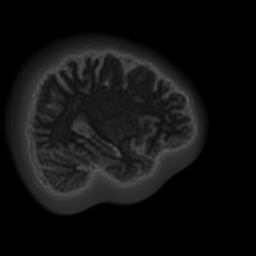
\includegraphics[width=0.22\linewidth]{imgs/3T_bilinear}
		\hskip\skipper
		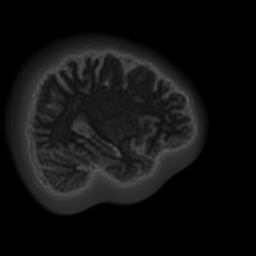
\includegraphics[width=0.22\linewidth]{imgs/3T_bilinear}
		\hskip\skipper
		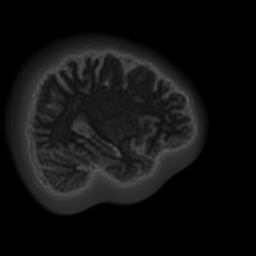
\includegraphics[width=0.22\linewidth]{imgs/3T_bilinear}
		%		\caption{1.5T and 3T respectively YZ MRI images after making kernel size divisible by stride.}
		%		\label{fig:troubleshootc}
	\end{subfigure}
	\vskip\ripper
	\begin{subfigure}[b]{0.7\textwidth}
		\centering
		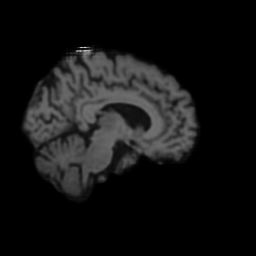
\includegraphics[width=0.22\linewidth]{imgs/1.5T_no_noise}
		\hskip\skipper
		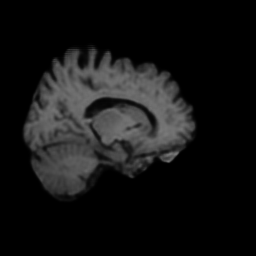
\includegraphics[width=0.22\linewidth]{imgs/3T_no_noise}
		\hskip\skipper
		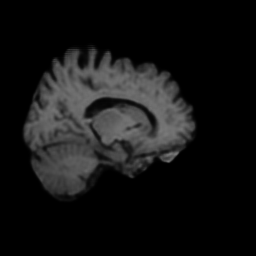
\includegraphics[width=0.22\linewidth]{imgs/3T_no_noise}
		\hskip\skipper
		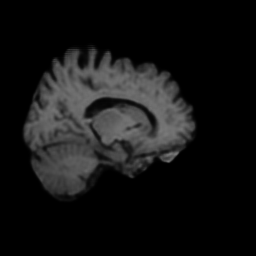
\includegraphics[width=0.22\linewidth]{imgs/3T_no_noise}
		%		\caption{1.5T and 3T respectively YZ MRI images after bilinear interpolation has been changed to nearest neighbor interpolation.}
		%		\label{fig:troubleshootd}
	\end{subfigure}
	\vskip\ripper
	\begin{subfigure}[b]{0.7\textwidth}
		\centering
		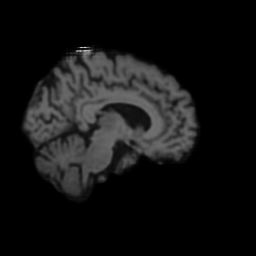
\includegraphics[width=0.22\linewidth]{imgs/1.5T_no_noise}
		\hskip\skipper
		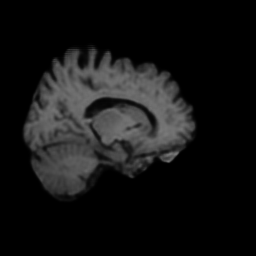
\includegraphics[width=0.22\linewidth]{imgs/3T_no_noise}
		\hskip\skipper
		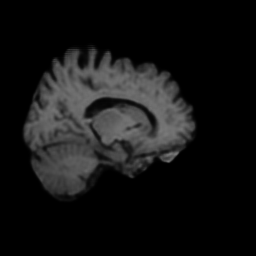
\includegraphics[width=0.22\linewidth]{imgs/3T_no_noise}
		\hskip\skipper
		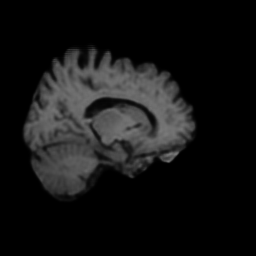
\includegraphics[width=0.22\linewidth]{imgs/3T_no_noise}
		%		\caption{1.5T and 3T respectively YZ MRI images after bilinear interpolation has been changed to nearest neighbor interpolation.}
		%		\label{fig:troubleshootd}
	\end{subfigure}
	\vskip\ripper
	\begin{subfigure}[b]{0.7\textwidth}
		\centering
		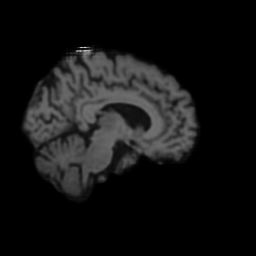
\includegraphics[width=0.22\linewidth]{imgs/1.5T_no_noise}
		\hskip\skipper
		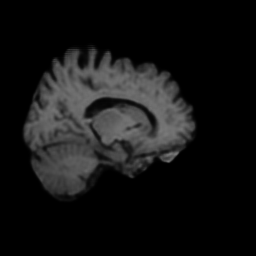
\includegraphics[width=0.22\linewidth]{imgs/3T_no_noise}
		\hskip\skipper
		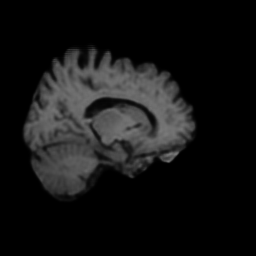
\includegraphics[width=0.22\linewidth]{imgs/3T_no_noise}
		\hskip\skipper
		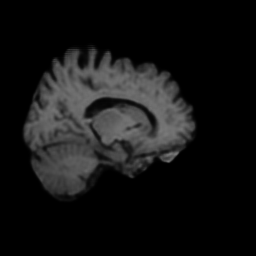
\includegraphics[width=0.22\linewidth]{imgs/3T_no_noise}
		%		\caption{1.5T and 3T respectively YZ MRI images after bilinear interpolation has been changed to nearest neighbor interpolation.}
		%		\label{fig:troubleshootd}
	\end{subfigure}
	%	\caption{Comparison of troubleshooting efforts to solve the visual issues in the generated images from the generators.}
	%	\label{fig:troubleshoot}
\end{figure}

\subsection{XZ Generated Images}\label{xz_generated}
%TODO: Fyld ud med de rigtige billeder og skriv figurtekst
%TODO: Her er tanken at rows eller columns indeholder ægte 3T, ægte 1.5T, reconstructed 3T og reconstructed 1.5T
\begin{figure}[H]
	\centering
	\begin{subfigure}[b]{0.7\textwidth}
		\centering
		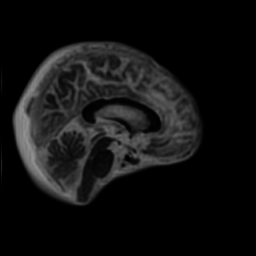
\includegraphics[width=0.22\linewidth]{imgs/1.5T_bilinear}
		\hskip\skipper
		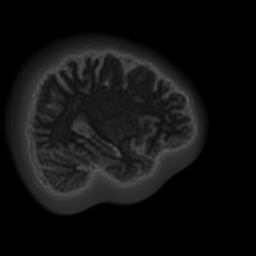
\includegraphics[width=0.22\linewidth]{imgs/3T_bilinear}
		\hskip\skipper
		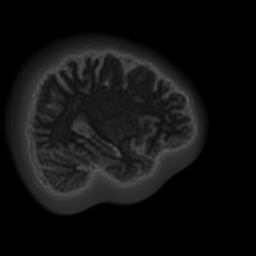
\includegraphics[width=0.22\linewidth]{imgs/3T_bilinear}
		\hskip\skipper
		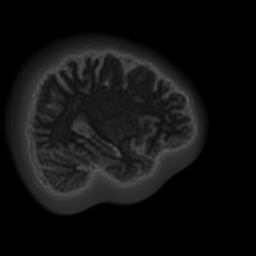
\includegraphics[width=0.22\linewidth]{imgs/3T_bilinear}
		%		\caption{1.5T and 3T respectively YZ MRI images after making kernel size divisible by stride.}
		%		\label{fig:troubleshootc}
	\end{subfigure}
	\vskip\ripper
	\begin{subfigure}[b]{0.7\textwidth}
		\centering
		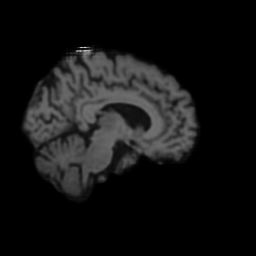
\includegraphics[width=0.22\linewidth]{imgs/1.5T_no_noise}
		\hskip\skipper
		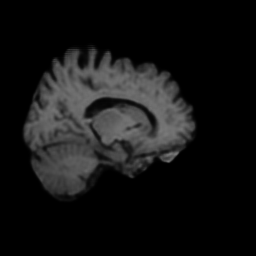
\includegraphics[width=0.22\linewidth]{imgs/3T_no_noise}
		\hskip\skipper
		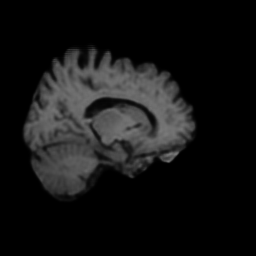
\includegraphics[width=0.22\linewidth]{imgs/3T_no_noise}
		\hskip\skipper
		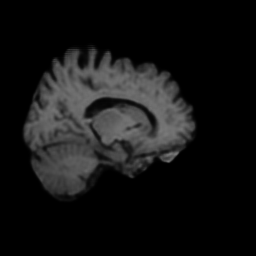
\includegraphics[width=0.22\linewidth]{imgs/3T_no_noise}
		%		\caption{1.5T and 3T respectively YZ MRI images after bilinear interpolation has been changed to nearest neighbor interpolation.}
		%		\label{fig:troubleshootd}
	\end{subfigure}
	\vskip\ripper
	\begin{subfigure}[b]{0.7\textwidth}
		\centering
		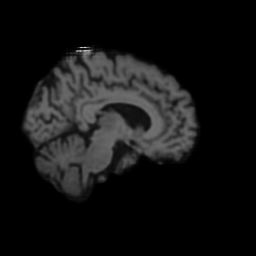
\includegraphics[width=0.22\linewidth]{imgs/1.5T_no_noise}
		\hskip\skipper
		\includegraphics[width=0.22\linewidth]{imgs/3T_no_noise}
		\hskip\skipper
		\includegraphics[width=0.22\linewidth]{imgs/3T_no_noise}
		\hskip\skipper
		\includegraphics[width=0.22\linewidth]{imgs/3T_no_noise}
		%		\caption{1.5T and 3T respectively YZ MRI images after bilinear interpolation has been changed to nearest neighbor interpolation.}
		%		\label{fig:troubleshootd}
	\end{subfigure}
	\vskip\ripper
	\begin{subfigure}[b]{0.7\textwidth}
		\centering
		\includegraphics[width=0.22\linewidth]{imgs/1.5T_no_noise}
		\hskip\skipper
		\includegraphics[width=0.22\linewidth]{imgs/3T_no_noise}
		\hskip\skipper
		\includegraphics[width=0.22\linewidth]{imgs/3T_no_noise}
		\hskip\skipper
		\includegraphics[width=0.22\linewidth]{imgs/3T_no_noise}
		%		\caption{1.5T and 3T respectively YZ MRI images after bilinear interpolation has been changed to nearest neighbor interpolation.}
		%		\label{fig:troubleshootd}
	\end{subfigure}
	%	\caption{Comparison of troubleshooting efforts to solve the visual issues in the generated images from the generators.}
	%	\label{fig:troubleshoot}
\end{figure}

\subsection{YZ Generated Images}\label{yz_generated}
%TODO: Fyld ud med de rigtige billeder og skriv figurtekst
%TODO: Her er tanken at rows eller columns indeholder ægte 3T, ægte 1.5T, reconstructed 3T og reconstructed 1.5T
\begin{figure}[H]
	\centering
	\begin{subfigure}[b]{0.7\textwidth}
		\centering
		\includegraphics[width=0.22\linewidth]{imgs/1.5T_bilinear}
		\hskip\skipper
		\includegraphics[width=0.22\linewidth]{imgs/3T_bilinear}
		\hskip\skipper
		\includegraphics[width=0.22\linewidth]{imgs/3T_bilinear}
		\hskip\skipper
		\includegraphics[width=0.22\linewidth]{imgs/3T_bilinear}
		%		\caption{1.5T and 3T respectively YZ MRI images after making kernel size divisible by stride.}
		%		\label{fig:troubleshootc}
	\end{subfigure}
	\vskip\ripper
	\begin{subfigure}[b]{0.7\textwidth}
		\centering
		\includegraphics[width=0.22\linewidth]{imgs/1.5T_no_noise}
		\hskip\skipper
		\includegraphics[width=0.22\linewidth]{imgs/3T_no_noise}
		\hskip\skipper
		\includegraphics[width=0.22\linewidth]{imgs/3T_no_noise}
		\hskip\skipper
		\includegraphics[width=0.22\linewidth]{imgs/3T_no_noise}
		%		\caption{1.5T and 3T respectively YZ MRI images after bilinear interpolation has been changed to nearest neighbor interpolation.}
		%		\label{fig:troubleshootd}
	\end{subfigure}
	\vskip\ripper
	\begin{subfigure}[b]{0.7\textwidth}
		\centering
		\includegraphics[width=0.22\linewidth]{imgs/1.5T_no_noise}
		\hskip\skipper
		\includegraphics[width=0.22\linewidth]{imgs/3T_no_noise}
		\hskip\skipper
		\includegraphics[width=0.22\linewidth]{imgs/3T_no_noise}
		\hskip\skipper
		\includegraphics[width=0.22\linewidth]{imgs/3T_no_noise}
		%		\caption{1.5T and 3T respectively YZ MRI images after bilinear interpolation has been changed to nearest neighbor interpolation.}
		%		\label{fig:troubleshootd}
	\end{subfigure}
	\vskip\ripper
	\begin{subfigure}[b]{0.7\textwidth}
		\centering
		\includegraphics[width=0.22\linewidth]{imgs/1.5T_no_noise}
		\hskip\skipper
		\includegraphics[width=0.22\linewidth]{imgs/3T_no_noise}
		\hskip\skipper
		\includegraphics[width=0.22\linewidth]{imgs/3T_no_noise}
		\hskip\skipper
		\includegraphics[width=0.22\linewidth]{imgs/3T_no_noise}
		%		\caption{1.5T and 3T respectively YZ MRI images after bilinear interpolation has been changed to nearest neighbor interpolation.}
		%		\label{fig:troubleshootd}
	\end{subfigure}
	%	\caption{Comparison of troubleshooting efforts to solve the visual issues in the generated images from the generators.}
	%	\label{fig:troubleshoot}
\end{figure}

\subsection{All Planes Generated Images}\label{all_generated}
%TODO: Fyld ud med de rigtige billeder og skriv figurtekst
%TODO: Her er tanken at rows eller columns indeholder ægte 3T, ægte 1.5T, reconstructed 3T og reconstructed 1.5T
\begin{figure}[H]
	\centering
	\begin{subfigure}[b]{0.7\textwidth}
		\centering
		\includegraphics[width=0.22\linewidth]{imgs/1.5T_bilinear}
		\hskip\skipper
		\includegraphics[width=0.22\linewidth]{imgs/3T_bilinear}
		\hskip\skipper
		\includegraphics[width=0.22\linewidth]{imgs/3T_bilinear}
		\hskip\skipper
		\includegraphics[width=0.22\linewidth]{imgs/3T_bilinear}
		%		\caption{1.5T and 3T respectively YZ MRI images after making kernel size divisible by stride.}
		%		\label{fig:troubleshootc}
	\end{subfigure}
	\vskip\ripper
	\begin{subfigure}[b]{0.7\textwidth}
		\centering
		\includegraphics[width=0.22\linewidth]{imgs/1.5T_no_noise}
		\hskip\skipper
		\includegraphics[width=0.22\linewidth]{imgs/3T_no_noise}
		\hskip\skipper
		\includegraphics[width=0.22\linewidth]{imgs/3T_no_noise}
		\hskip\skipper
		\includegraphics[width=0.22\linewidth]{imgs/3T_no_noise}
		%		\caption{1.5T and 3T respectively YZ MRI images after bilinear interpolation has been changed to nearest neighbor interpolation.}
		%		\label{fig:troubleshootd}
	\end{subfigure}
	\vskip\ripper
	\begin{subfigure}[b]{0.7\textwidth}
		\centering
		\includegraphics[width=0.22\linewidth]{imgs/1.5T_no_noise}
		\hskip\skipper
		\includegraphics[width=0.22\linewidth]{imgs/3T_no_noise}
		\hskip\skipper
		\includegraphics[width=0.22\linewidth]{imgs/3T_no_noise}
		\hskip\skipper
		\includegraphics[width=0.22\linewidth]{imgs/3T_no_noise}
		%		\caption{1.5T and 3T respectively YZ MRI images after bilinear interpolation has been changed to nearest neighbor interpolation.}
		%		\label{fig:troubleshootd}
	\end{subfigure}
	\vskip\ripper
	\begin{subfigure}[b]{0.7\textwidth}
		\centering
		\includegraphics[width=0.22\linewidth]{imgs/1.5T_no_noise}
		\hskip\skipper
		\includegraphics[width=0.22\linewidth]{imgs/3T_no_noise}
		\hskip\skipper
		\includegraphics[width=0.22\linewidth]{imgs/3T_no_noise}
		\hskip\skipper
		\includegraphics[width=0.22\linewidth]{imgs/3T_no_noise}
		%		\caption{1.5T and 3T respectively YZ MRI images after bilinear interpolation has been changed to nearest neighbor interpolation.}
		%		\label{fig:troubleshootd}
	\end{subfigure}
	%	\caption{Comparison of troubleshooting efforts to solve the visual issues in the generated images from the generators.}
	%	\label{fig:troubleshoot}
\end{figure}

\subsection{Discriminator Losses}\label{disc_loss}
%TODO: Fyld ud med de rigtige billeder og skriv figurtekst
\begin{figure}[H]
	\centering
	\begin{subfigure}[b]{0.8\textwidth}
		\centering
		\includegraphics[width=\linewidth]{imgs/placeholder_discriminator_losses}
		\hfill
		\includegraphics[width=\linewidth]{imgs/placeholder_discriminator_losses}
		\hfill
		\includegraphics[width=\linewidth]{imgs/placeholder_discriminator_losses}
		\hfill
		\includegraphics[width=\linewidth]{imgs/placeholder_discriminator_losses}
%		\caption{1.5T and 3T respectively YZ MRI images after bilinear interpolation has been implemented in upsampling.}
%		\label{fig:troubleshootb}
	\end{subfigure}
%	\caption{text}
%	\label{key}
\end{figure}

\subsection{Generator Losses}\label{gen_loss}
%TODO: Fyld ud med de rigtige billeder og skriv figurtekst
\begin{figure}[H]
	\centering
	\begin{subfigure}[b]{0.8\textwidth}
		\centering
		\includegraphics[width=\linewidth]{imgs/placeholder_generator_losses}
		\hfill
		\includegraphics[width=\linewidth]{imgs/placeholder_generator_losses}
		\hfill
		\includegraphics[width=\linewidth]{imgs/placeholder_generator_losses}
		\hfill
		\includegraphics[width=\linewidth]{imgs/placeholder_generator_losses}
		%		\caption{1.5T and 3T respectively YZ MRI images after bilinear interpolation has been implemented in upsampling.}
		%		\label{fig:troubleshootb}
	\end{subfigure}
	%	\caption{text}
	%	\label{key}
\end{figure}

\subsection{Cycle-Consistency Losses}\label{cycle_loss}
%TODO: Fyld ud med de rigtige billeder og skriv figurtekst
\begin{figure}[H]
	\centering
	\begin{subfigure}[b]{0.8\textwidth}
		\centering
		\includegraphics[width=\linewidth]{imgs/placeholder_cycle_losses}
		\hfill
		\includegraphics[width=\linewidth]{imgs/placeholder_cycle_losses}
		\hfill
		\includegraphics[width=\linewidth]{imgs/placeholder_cycle_losses}
		\hfill
		\includegraphics[width=\linewidth]{imgs/placeholder_cycle_losses}
		%		\caption{1.5T and 3T respectively YZ MRI images after bilinear interpolation has been implemented in upsampling.}
		%		\label{fig:troubleshootb}
	\end{subfigure}
	%	\caption{text}
	%	\label{key}
\end{figure}

\subsection{Identity Losses}\label{iden_loss}
%TODO: Fyld ud med de rigtige billeder og skriv figurtekst
\begin{figure}[H]
	\centering
	\begin{subfigure}[b]{0.8\textwidth}
		\centering
		\includegraphics[width=\linewidth]{imgs/placeholder_identity_losses}
		\hfill
		\includegraphics[width=\linewidth]{imgs/placeholder_identity_losses}
		\hfill
		\includegraphics[width=\linewidth]{imgs/placeholder_identity_losses}
		\hfill
		\includegraphics[width=\linewidth]{imgs/placeholder_identity_losses}
		%		\caption{1.5T and 3T respectively YZ MRI images after bilinear interpolation has been implemented in upsampling.}
		%		\label{fig:troubleshootb}
	\end{subfigure}
	%	\caption{text}
	%	\label{key}
\end{figure}



\section{Discussion}\label{discussion}


\subsection{What do the Results Show?}\label{discussionOfResults}


\subsection{Would the Model be Efficacious in Practice?}


\subsection{Standardization of Measuring Equipment (3T/1.5T)}


\subsection{Improvements for Future Papers}


\subsection{Dealing With GDPR in Personal Data}


\subsection{Safe AI}


\subsection{Economic Incentive of a good classification model}

One could ask the question of what societal and economic implications a good classification model within this field study could imply. This section aims to estimate the outcome of implementing such a classifier into the society of Denmark. This will give an insight into whether continuing to study in this field would make sense for the sake of societal impact. The danish 2025 dementia plan has the following goals:

\begin{itemize}
	\item Denmark needs 98 dementia friendly communes
	\item 80 \% of people with dementia needs a specific diagnosis 
	\item Reduce the amount of anti-psychotic medicine with 50 \% in year 2025
\end{itemize}
\noindent
One of the relevant key focus areas include early detection and quality treatment which can be aided by the deep learning models. An average patient with dementia cost approximately $ 51000 \ \texttt{DKK / year}$:

%\texttt{\begin{table}
		%	\item Practice sector: 3900 DKK
		%	\item Hospital sector somatics: 33500 DKK 
		%	\item Hospital psychiatry: 4000 DKK
		%	\item Medicine: 9700 DKK 
		%\end{table}}
		
		\begin{table}[H]
			\begin{tabular}{ll}
				Practice sector   &\ \ 3900  DKK  \\
				Hospital sector somatics  & 33500 DKK \\
				Hospital psychiatry  &  \ \ 4000  DKK  \\
				Medicine & \ \ 9700  DKK 
			\end{tabular}
		\end{table}
		
		In Denmark around $ 85000-90000 $ people live with a dementia disease. Around 50000 of these cases are Alzheimer. Every year around $ 8000 $ new cases are detected and in 2040 the expected amount of people with dementia above 60 years old is $ 125000 $ to $ 150000 $. This amount to Denmark spending $ 4.59 $ Billion DKK / year on Alzheimer Patients to $ 7.65 $ Billion DKK / year. \footnote{!NB Not taking inflation into consideration for the outlined numbers} These numbers do not take healthcare personal, researchers and other variable costs into consideration. Moreover, 65\% to 85\% of all inhabitants in eldercare has a dementia disease. The cost of informal care time ranges between $ 5.0 $ to $ 6.9 $ hours daily. Furthermore, the daily cost was estimated to range between $ 1190 - 1658 $ DKK / day for primary caregivers\footnote{A primary caregiver can range from everything from a nurse, family member etc.} and $ 171 - 253 $ DKK / day for secondary caregivers. The cost for Denmark amounts to $ 18 $ Billion DKK / year, on eldercare alone. The total cost of dementia related diseases in Denmark is estimated to be 20 Billion DKK / year.  \cite{Alzheimerforeningen} \cite{informal_care} Thus, a screening to detect Alzheimer before a patient showing symptoms can be a way to both drive down cost of the danish society, but also optimize life expectancy and quality for the citizens of Denmark.
		
		% TODO: inkluder sygeplejerske


\section{Conclusion}\label{conclusion}



\newpage
\section{Appendix}\label{appendix}


\subsection{Breakdown of Code}


\subsection{Shell scripts}


\subsection{MNIST GAN}
%TODO: Skriv en introduktion til denne section

\subsubsection{Losses}

\begin{figure}[H]
	\centering
	\begin{subfigure}[b]{0.9\textwidth}
		\centering
		\includegraphics[width=\linewidth]{imgs/MNIST_GAN_normal_losses}
		\hfill
		\includegraphics[width=\linewidth]{imgs/MNIST_GAN_mse_losses}
	\end{subfigure}
	\caption{The losses measured two times each epoch for 200 epochs during training of the GAN on the MNIST dataset. \textbf{Top:} Training the model using L1 loss for the discriminator and BCE with logits loss for the generator. \textbf{Bottom:} Training the model using MSE loss for both models. MSE has a tendency to generally work well when training neural networks.}
	\label{fig:MNIST_GAN_losses}
\end{figure}

\subsubsection{Progress of Training}

\begin{figure}[H]
	\centering
	\includegraphics[width=\linewidth]{imgs/MNIST_GAN_normal_result_epoch_0_minibatch_500}
	\hfill
	\includegraphics[width=\linewidth]{imgs/MNIST_GAN_normal_result_epoch_68_minibatch_0}
\end{figure}
\begin{figure}[H]
	\includegraphics[width=\linewidth]{imgs/MNIST_GAN_normal_result_epoch_148_minibatch_0}
	\hfill
	\includegraphics[width=\linewidth]{imgs/MNIST_GAN_normal_result_epoch_198_minibatch_500}
	\caption{During training, 11 random generated images have been shown at different points along the training process (epoch 2, epoch 70, epoch 150 and epoch 200). The epochs were chosen to show the most interesting behavior or the achieved best performance of the model. The last of the 12 plots depicts the discriminator prediction for the current minibatch. The red columns are generated images and green columns are real images. as such, a perfect discriminator would place every red column at 0 and every green column at 1.}
	\label{fig:training_progress_normal}
\end{figure}

\begin{figure}[H]
	\centering
	\includegraphics[width=\linewidth]{imgs/MNIST_GAN_mse_result_epoch_1_minibatch_0}
	\hfill
	\includegraphics[width=\linewidth]{imgs/MNIST_GAN_mse_result_epoch_13_minibatch_0}
\end{figure}
\begin{figure}[H]
	\includegraphics[width=\linewidth]{imgs/MNIST_GAN_mse_result_epoch_84_minibatch_500}
	\hfill
	\includegraphics[width=\linewidth]{imgs/MNIST_GAN_mse_result_epoch_195_minibatch_0}
	\caption{During training, 11 random generated images have been shown at different points along the training process (epoch 3, epoch 15, epoch 86 and epoch 197). The epochs were chosen to show the most interesting behavior or the achieved best performance of the model. The last of the 12 plots depicts the discriminator prediction for the current minibatch. The red columns are generated images and green columns are real images. as such, a perfect discriminator would place every red column at 0 and every green column at 1.}
		\label{fig:training_progress_mse}
\end{figure}

\subsubsection{Generated Images}
%TODO: skriv figurtekst
\begin{figure}[H]
	\centering
	\begin{subfigure}[b]{0.7\textwidth}
		\centering
		\includegraphics[width=0.22\linewidth]{imgs/MNIST_GAN_normal_real_0}
		\hskip\skipper
		\includegraphics[width=0.22\linewidth]{imgs/MNIST_GAN_normal_fake_0}
		\hskip\skipper
		\includegraphics[width=0.22\linewidth]{imgs/MNIST_GAN_normal_real_1}
		\hskip\skipper
		\includegraphics[width=0.22\linewidth]{imgs/MNIST_GAN_normal_fake_1}
	\end{subfigure}
	\vskip\ripper
	\begin{subfigure}[b]{0.7\textwidth}
		\centering
		\includegraphics[width=0.22\linewidth]{imgs/MNIST_GAN_normal_real_2}
		\hskip\skipper
		\includegraphics[width=0.22\linewidth]{imgs/MNIST_GAN_normal_fake_2}
		\hskip\skipper
		\includegraphics[width=0.22\linewidth]{imgs/MNIST_GAN_normal_real_3}
		\hskip\skipper
		\includegraphics[width=0.22\linewidth]{imgs/MNIST_GAN_normal_fake_3}
	\end{subfigure}
	\vskip\ripper
	\begin{subfigure}[b]{0.7\textwidth}
		\centering
		\includegraphics[width=0.22\linewidth]{imgs/MNIST_GAN_normal_real_4}
		\hskip\skipper
		\includegraphics[width=0.22\linewidth]{imgs/MNIST_GAN_normal_fake_4}
		\hskip\skipper
		\includegraphics[width=0.22\linewidth]{imgs/MNIST_GAN_normal_real_5}
		\hskip\skipper
		\includegraphics[width=0.22\linewidth]{imgs/MNIST_GAN_normal_fake_5}
	\end{subfigure}
	\vskip\ripper
	\begin{subfigure}[b]{0.7\textwidth}
		\centering
		\includegraphics[width=0.22\linewidth]{imgs/MNIST_GAN_normal_real_6}
		\hskip\skipper
		\includegraphics[width=0.22\linewidth]{imgs/MNIST_GAN_normal_fake_6}
		\hskip\skipper
		\includegraphics[width=0.22\linewidth]{imgs/MNIST_GAN_normal_real_7}
		\hskip\skipper
		\includegraphics[width=0.22\linewidth]{imgs/MNIST_GAN_normal_fake_7}
	\end{subfigure}
	\caption{Samples of real images from the MNIST dataset of handwritten digits and generated images from the generator in the MNIST GAN using L1 loss and BCE. Column 1 and 3 show real images and column 2 and 4 show generated images.}
	\label{fig:generated_images_MNIST_GAN_normal}
\end{figure}

%TODO: skriv figurtekst
\begin{figure}[H]
	\centering
	\begin{subfigure}[b]{0.7\textwidth}
		\centering
		\includegraphics[width=0.22\linewidth]{imgs/MNIST_GAN_mse_real_0}
		\hskip\skipper
		\includegraphics[width=0.22\linewidth]{imgs/MNIST_GAN_mse_fake_0}
		\hskip\skipper
		\includegraphics[width=0.22\linewidth]{imgs/MNIST_GAN_mse_real_1}
		\hskip\skipper
		\includegraphics[width=0.22\linewidth]{imgs/MNIST_GAN_mse_fake_1}
	\end{subfigure}
	\vskip\ripper
	\begin{subfigure}[b]{0.7\textwidth}
		\centering
		\includegraphics[width=0.22\linewidth]{imgs/MNIST_GAN_mse_real_2}
		\hskip\skipper
		\includegraphics[width=0.22\linewidth]{imgs/MNIST_GAN_mse_fake_2}
		\hskip\skipper
		\includegraphics[width=0.22\linewidth]{imgs/MNIST_GAN_mse_real_3}
		\hskip\skipper
		\includegraphics[width=0.22\linewidth]{imgs/MNIST_GAN_mse_fake_3}
	\end{subfigure}
	\vskip\ripper
	\begin{subfigure}[b]{0.7\textwidth}
		\centering
		\includegraphics[width=0.22\linewidth]{imgs/MNIST_GAN_mse_real_4}
		\hskip\skipper
		\includegraphics[width=0.22\linewidth]{imgs/MNIST_GAN_mse_fake_4}
		\hskip\skipper
		\includegraphics[width=0.22\linewidth]{imgs/MNIST_GAN_mse_real_5}
		\hskip\skipper
		\includegraphics[width=0.22\linewidth]{imgs/MNIST_GAN_mse_fake_5}
	\end{subfigure}
	\vskip\ripper
	\begin{subfigure}[b]{0.7\textwidth}
		\centering
		\includegraphics[width=0.22\linewidth]{imgs/MNIST_GAN_mse_real_6}
		\hskip\skipper
		\includegraphics[width=0.22\linewidth]{imgs/MNIST_GAN_mse_fake_6}
		\hskip\skipper
		\includegraphics[width=0.22\linewidth]{imgs/MNIST_GAN_mse_real_7}
		\hskip\skipper
		\includegraphics[width=0.22\linewidth]{imgs/MNIST_GAN_mse_fake_7}
	\end{subfigure}
	\caption{Samples of real images from the MNIST dataset of handwritten digits and generated images from the generator in the MNIST GAN using MSE loss. Column 1 and 3 show real images and column 2 and 4 show generated images.}
	\label{fig:generated_images_MNIST_GAN_mse}
\end{figure}

%TODO: Vis hvor god discriminatoren er blevet

\subsubsection{Discussion of Results}
%TODO: Skriv om resultaterne og årsagerne til dem


\subsection{Horse2Zebra CycleGAN}


\subsubsection{Losses}

%TODO: Fyld ud med de rigtige billeder og skriv figurtekst
%TODO: Tanken er at denne figure indeholder alle fire losses. Ellers kan de opdeles med hver deres figurtekst
\begin{figure}[H]
	\centering
	\begin{subfigure}[b]{0.8\textwidth}
		\centering
		\includegraphics[width=\linewidth]{imgs/placeholder_identity_losses}
		\hfill
		\includegraphics[width=\linewidth]{imgs/placeholder_identity_losses}
		\hfill
		\includegraphics[width=\linewidth]{imgs/placeholder_identity_losses}
		\hfill
		\includegraphics[width=\linewidth]{imgs/placeholder_identity_losses}
		%		\caption{1.5T and 3T respectively YZ MRI images after bilinear interpolation has been implemented in upsampling.}
		%		\label{fig:troubleshootb}
	\end{subfigure}
	%	\caption{text}
	%	\label{key}
\end{figure}

\subsubsection{Progress of Training}

%TODO: Fyld ud med de rigtige billeder og skriv figurtekst
%TODO: vis hvordan billederne bliver bedre over tid og vis eksempler på heste
\begin{figure}[H]
	\centering
	\begin{subfigure}[b]{0.7\textwidth}
		\centering
		\includegraphics[width=0.22\linewidth]{imgs/temp_horse}
		\hskip\skipper
		\includegraphics[width=0.22\linewidth]{imgs/temp_horse}
		\hskip\skipper
		\includegraphics[width=0.22\linewidth]{imgs/temp_horse}
		\hskip\skipper
		\includegraphics[width=0.22\linewidth]{imgs/temp_horse}
		%		\caption{1.5T and 3T respectively YZ MRI images after making kernel size divisible by stride.}
		%		\label{fig:troubleshootc}
	\end{subfigure}
	\vskip\ripper
	\begin{subfigure}[b]{0.7\textwidth}
		\centering
		\includegraphics[width=0.22\linewidth]{imgs/temp_horse}
		\hskip\skipper
		\includegraphics[width=0.22\linewidth]{imgs/temp_horse}
		\hskip\skipper
		\includegraphics[width=0.22\linewidth]{imgs/temp_horse}
		\hskip\skipper
		\includegraphics[width=0.22\linewidth]{imgs/temp_horse}
		%		\caption{1.5T and 3T respectively YZ MRI images after bilinear interpolation has been changed to nearest neighbor interpolation.}
		%		\label{fig:troubleshootd}
	\end{subfigure}
	\vskip\ripper
	\begin{subfigure}[b]{0.7\textwidth}
		\centering
		\includegraphics[width=0.22\linewidth]{imgs/temp_horse}
		\hskip\skipper
		\includegraphics[width=0.22\linewidth]{imgs/temp_horse}
		\hskip\skipper
		\includegraphics[width=0.22\linewidth]{imgs/temp_horse}
		\hskip\skipper
		\includegraphics[width=0.22\linewidth]{imgs/temp_horse}
		%		\caption{1.5T and 3T respectively YZ MRI images after bilinear interpolation has been changed to nearest neighbor interpolation.}
		%		\label{fig:troubleshootd}
	\end{subfigure}
	\vskip\ripper
	\begin{subfigure}[b]{0.7\textwidth}
		\centering
		\includegraphics[width=0.22\linewidth]{imgs/temp_horse}
		\hskip\skipper
		\includegraphics[width=0.22\linewidth]{imgs/temp_horse}
		\hskip\skipper
		\includegraphics[width=0.22\linewidth]{imgs/temp_horse}
		\hskip\skipper
		\includegraphics[width=0.22\linewidth]{imgs/temp_horse}
		%		\caption{1.5T and 3T respectively YZ MRI images after bilinear interpolation has been changed to nearest neighbor interpolation.}
		%		\label{fig:troubleshootd}
	\end{subfigure}
	%	\caption{Comparison of troubleshooting efforts to solve the visual issues in the generated images from the generators.}
	%	\label{fig:troubleshoot}
\end{figure}


%TODO: Fyld ud med de rigtige billeder og skriv figurtekst
%TODO: vis hvordan billederne bliver bedre over tid og vis eksempler på zebraer
\begin{figure}[H]
	\centering
	\begin{subfigure}[b]{0.7\textwidth}
		\centering
		\includegraphics[width=0.22\linewidth]{imgs/temp_zebra}
		\hskip\skipper
		\includegraphics[width=0.22\linewidth]{imgs/temp_zebra}
		\hskip\skipper
		\includegraphics[width=0.22\linewidth]{imgs/temp_zebra}
		\hskip\skipper
		\includegraphics[width=0.22\linewidth]{imgs/temp_zebra}
		%		\caption{1.5T and 3T respectively YZ MRI images after making kernel size divisible by stride.}
		%		\label{fig:troubleshootc}
	\end{subfigure}
	\vskip\ripper
	\begin{subfigure}[b]{0.7\textwidth}
		\centering
		\includegraphics[width=0.22\linewidth]{imgs/temp_zebra}
		\hskip\skipper
		\includegraphics[width=0.22\linewidth]{imgs/temp_zebra}
		\hskip\skipper
		\includegraphics[width=0.22\linewidth]{imgs/temp_zebra}
		\hskip\skipper
		\includegraphics[width=0.22\linewidth]{imgs/temp_zebra}
		%		\caption{1.5T and 3T respectively YZ MRI images after bilinear interpolation has been changed to nearest neighbor interpolation.}
		%		\label{fig:troubleshootd}
	\end{subfigure}
	\vskip\ripper
	\begin{subfigure}[b]{0.7\textwidth}
		\centering
		\includegraphics[width=0.22\linewidth]{imgs/temp_zebra}
		\hskip\skipper
		\includegraphics[width=0.22\linewidth]{imgs/temp_zebra}
		\hskip\skipper
		\includegraphics[width=0.22\linewidth]{imgs/temp_zebra}
		\hskip\skipper
		\includegraphics[width=0.22\linewidth]{imgs/temp_zebra}
		%		\caption{1.5T and 3T respectively YZ MRI images after bilinear interpolation has been changed to nearest neighbor interpolation.}
		%		\label{fig:troubleshootd}
	\end{subfigure}
	\vskip\ripper
	\begin{subfigure}[b]{0.7\textwidth}
		\centering
		\includegraphics[width=0.22\linewidth]{imgs/temp_zebra}
		\hskip\skipper
		\includegraphics[width=0.22\linewidth]{imgs/temp_zebra}
		\hskip\skipper
		\includegraphics[width=0.22\linewidth]{imgs/temp_zebra}
		\hskip\skipper
		\includegraphics[width=0.22\linewidth]{imgs/temp_zebra}
		%		\caption{1.5T and 3T respectively YZ MRI images after bilinear interpolation has been changed to nearest neighbor interpolation.}
		%		\label{fig:troubleshootd}
	\end{subfigure}
	%	\caption{Comparison of troubleshooting efforts to solve the visual issues in the generated images from the generators.}
	%	\label{fig:troubleshoot}
\end{figure}

\subsubsection{Discussion of Results}
%TODO: Skriv om resultaterne og årsagerne til dem


\newpage
\begin{thebibliography}{9} 
	
%	\bibitem{tv2} K. Andreasen "Flere end 15.000 deltog i dansk Black Lives Matter-demonstration", 2020 Tv2 Lorry, at \url{https://www.tv2lorry.dk/koebenhavn/15000-mennesker-samles-til-dansk-demonstration-mod-racisme-mod-racisme}, visited 19-06-2020
	
%	\bibitem{cnn1}  M. Macaya et al. "June 17 Black Lives Matter protests news", 2020 CNN, at \url{https://edition.cnn.com/us/live-news/black-lives-matter-protests-06-17-2020/index.html}, visited at 19-06-2020
	
%	\bibitem{cnn2} M. Macaya et al. "June 18 Black Lives Matter protests news", 2020 CNN, at \url{https://edition.cnn.com/us/live-news/black-lives-matter-protests-06-18-2020/index.html}, visited 19-06-2020
		
		
		\bibitem{first} Zhu, Jun-Yan, et al. "Unpaired image-to-image translation using cycle-consistent adversarial networks." Proceedings of the IEEE international conference on computer vision. 2017.
		
		\bibitem{second} Burns, Jeffrey M., et al. "Reduced lean mass in early Alzheimer disease and its association with brain atrophy." Archives of neurology 67.4 (2010): 428-433.
		
		\bibitem{CamillaKandidat} Pedersen, Camilla Kergel "Demographic bias in public neuroimaging databases, and its effect on AI systems for computer-aided diagnosis." University of Copenhagen Faculty of Science. 2021.
		
		\bibitem{adni}  Alzheimer’s
		Disease Neuroimaging Initiative homepage: \url{http://adni.loni.usc.edu/}, last visited at 
		28 Nov. 2021
		
		\bibitem{adni1} Alzheimer’s
		Disease Neuroimaging Initiative about ADNI1 \url{http://adni.loni.usc.edu/about/adni1/}, last visited at 28 Nov. 2021
		
		\bibitem{freesurfer} FreeSurfer Software Suite \url{https://surfer.nmr.mgh.harvard.edu/}, last visited at 2nd December, 2021
		
		\bibitem{normalize} FreeSurfer: mri\_normalize, \url{https://surfer.nmr.mgh.harvard.edu/fswiki/mri_normalize}
		
		\bibitem{neuro} Basaia, Silvia et al. "Automated classification of alzheimer’s disease and mild cognitive impairment using a
		single mri and deep neural networks." NeuroImage: Clinical, 21:101645, 2019.
		
		\bibitem{suk_and_shen_1} 
		 Suk, Heung-II and Shen, Dinggang
		 "Deep learning-based feature representation for AD/MCI classification2", 2013
		 
		 \bibitem{suk_and_shen_2} Suk, Heung-II et al. "Latent feature representation with stacked auto-encoder for AD/MCI diagnosis", 2015
		
		\bibitem{cheng} Cheng, Danni "CNNs based multi-modality classification for AD diagnosis", 2017 10th International Congress on Image and Signal Processing, BioMedical Engineering and Informatics (CISP-BMEI) 
		
		\bibitem{yudong} Zhang, Yudong et al. "C	lassification of Alzheimer Disease Based on Structural Magnetic
		Resonance Imaging by Kernel Support Vector Machine Decision Tree", Progress In Electromagnetics Research, Vol. 144, 171-184, 2014
		
		\bibitem{bcewithlogits} Paszke, A et al. "PyTorch: An Imperative Style, High-Performance Deep Learning Library", Curran Associates, Inc., 2019, https://pytorch.org/docs/stable/generated/torch.nn.BCEWithLogitsLoss.html
		
		\bibitem{ganlocalminimum} Bansal, Aayush et al. "Recycle-GAN: Unsupervised Video Retargeting", Carnegie Mellon University, 2018, https://arxiv.org/pdf/1808.05174.pdf
		
		\bibitem{checkerboard} Odena, et al., "Deconvolution and Checkerboard Artifacts", Distill, 2016. http://doi.org/10.23915/distill.00003
		
		\bibitem{learnableKernel} Neda et al., "torch.nn.ConvTranspose2d vs torch.nn.Upsample", PyTorch, 2018. https://discuss.pytorch.org/t/torch-nn-convtranspose2d-vs-torch-nn-upsample/30574/7
		
		\bibitem{Alzheimerforeningen} Alzheimer.dk "Fakta om demens": \url{https://www.alzheimer.dk/viden-om-demens/fakta-om-demens/}, last visited at 22nd December, 2021
		
		\bibitem{informal_care} Jakobsen, Marie et al. "Costs of Informal Care for People Suffering from Dementia: Evidence from a Danish Survey"
		
		\bibitem{mode_collapse_MLM} Brownlee, Jason, "How to Identify and Diagnose GAN Failure Modes", Machine Learning Mastery, 2019, https://machinelearningmastery.com/practical-guide-to-gan-failure-modes/
		
		\bibitem{mode_collapse_reddit_fix} AnvaMiba, "[Discussion] Discriminator converging to 0 loss in very few steps while training GAN.", Reddit, 2016, https://www.reddit.com/r/MachineLearning/comments/5asl74/discussion\_discriminator\_converging\_to\_0\_loss\_in/
		
		\bibitem{mode_collapse_github} vrao9, "Loss D goes to zero when adding a new loss to generator", Github Issues, 2019, https://github.com/junyanz/pytorch-CycleGAN-and-pix2pix/issues/626
		
		\bibitem{hard_to_train} Hui, Jonathan, "GAN — Why it is so hard to train Generative Adversarial Networks!", Medium, 2018, https://jonathan-hui.medium.com/gan-why-it-is-so-hard-to-train-generative-advisory-networks-819a86b3750b
		
	\end{thebibliography}
	
	
	\newpage
	\bibliographystyle{IEEEbib}
	\bibliography{refs}
	
	
	
	% List of articles
	% Machine learning framework for early MRI-based Alzheimer's conversion prediction in MCI subjects - Elahi Mohadi et al
	% How early can we predict Alzheimer's disease using computational anatomy? - Stanisław Adaszewski
	%
	%
	%
	
\end{document}